\documentclass[letterpaper,10pt,draft]{book}
\usepackage[
  paper=letterpaper,
  lmargin=1in,
  rmargin=1in,
  tmargin=1in,
  bmargin=1in]{geometry}

%Uncomment below in the future to add indecies

% for adding index. Use \index{key} to put index keywords.
%\usepackage{multind}
%\makeindex{keyword}
%\makeindex{python}
%\makeindex{ui}

\newcommand{\mytitle}{\textbf{RGG User's Guide}}

% Make fancy headers and everything...
\usepackage{fancyhdr}
\pagestyle{fancy}
% Headers - left, center and right.
\lhead{}
\chead{\mytitle}
\rhead{}
% Footers - as before
%\lfoot{\scriptsize \emph{\svnInfoFile}}
\cfoot{\small \thepage}
%\rfoot{\scriptsize \emph{Rev: \svnInfoRevision , \svnInfoDate}}
\renewcommand{\headrulewidth}{0.5pt}
\renewcommand{\footrulewidth}{0.5pt}

%\addtolength{\headheight}{0.5pt} % make space for the rule
\setlength{\headheight}{14pt}
\fancypagestyle{plain}{%
  \fancyhead{} % get rid of headers on plain pages
  \renewcommand{\headrulewidth}{0pt} % and the line
}

% Remove indents, add line breaks after paragraphs.
\usepackage[parfill]{parskip}

% Now to define several macros for commonly used abbreviations and such
\usepackage{xspace}
\newcommand{\fixme}[1]{\footnote{{\color{red}#1}}}
\newcommand{\note}[1]{{\small\color{blue}[#1]}}
\newcommand{\todo}[1]{{\large\color{red}[TODO: #1]}}

\usepackage{url}
% Use in the form \url{http://mysite.co.uk/~marcus/} or \url!http://mysite.co.uk/~marcus/!

\usepackage[pdftex,final]{graphicx}
\usepackage[pdftex]{color}
\usepackage{setspace}

\usepackage{caption}
\usepackage{subcaption}

\usepackage{wrapfig}
\usepackage{float}


\usepackage{colortbl}
% 21st century - make some real links in the PDF, but keep the colors reasonable...
\usepackage[colorlinks=true,urlcolor=blue,citecolor=black,linkcolor=black,final=true]{hyperref}


%Inlcuding LatexMacros -- a borrowed subset from the Paraview User's Guide.
% Collection of macros and stuff to use in the user-guide.

%-------------------------------------------------------------------------------
% stuff for "boxed text" used for didyouknow and common error boxes.
%-------------------------------------------------------------------------------
\usepackage[tikz]{bclogo}
\usepackage[framemethod=tikz]{mdframed}

\definecolor{bgblue}{RGB}{245,243,253}
\definecolor{ttblue}{RGB}{91,194,224}


% change title color.
\renewcommand\bcStyleTitre[1]{\large\textcolor{ttblue}{#1}}
%\begin{bclogo}[couleur=bgblue, arrondi =0 , logo=\bcbombe, barre=none,noborder=true]{Commom Programming Error}
%\itshape\lipsum[4]
%\end{bclogo}

\newenvironment{commonerrors}%
{\vspace{1em}\begin{bclogo}[couleur=bgblue, arrondi =0 , logo=\bcbombe, barre=snake,noborder=true]{Common Errors}\itshape}%
{\end{bclogo}\vspace{1em}}

\newenvironment{didyouknow}%
{\vspace{1em}\begin{bclogo}[couleur=bgblue, arrondi =0 , logo=\bcinfo, barre=snake,noborder=true]{Did you know?}\itshape}%
{\end{bclogo}\vspace{1em}}


%-------------------------------------------------------------------------------
% Use this when referring to a menu e.g. \menu{Sources} or
% \menu{Sources}[Sphere]
%-------------------------------------------------------------------------------
\usepackage{xparse}
\DeclareDocumentCommand \menu {m o}
{%
  \IfNoValueTF{#2}%
    {\menuii{#1}}%
    {\menuii{#1}$\rightarrow$\menuii{#2}}%
}
%  {>{\SplitList{;}}m}
%  {\menuii #1 $\rightarrow$}
\newcommand\menuii[1]{\textbf{#1}}

%-------------------------------------------------------------------------------
% Use this when referring to a key sequence e.g. \key{Ctrl+F}.
%-------------------------------------------------------------------------------
\newcommand\key[1]{\texttt{#1}}

%-------------------------------------------------------------------------------
% Use this when referring to an entity on the UI. When referring to any text
% that appears on the ParaView UI, e.g. Pipeline Browser, Solid Color, etc. use
% this format e.g. \ui{Properties} panel, \ui{Pipeline Browser}.
%-------------------------------------------------------------------------------
\newcommand\ui[1]{\texttt{#1}\index{ui}{#1}}

%-------------------------------------------------------------------------------
% Use this when referring to executables e.g. \executable{paraview}
%-------------------------------------------------------------------------------
\newcommand\executable[1]{{\emph{\color{blue}#1}}}

%-------------------------------------------------------------------------------
% Use for keywords.
%-------------------------------------------------------------------------------
\newcommand\keyword[1]{\index{keyword}{#1}}

%-------------------------------------------------------------------------------
% Use for icons inlined in text e.g. ...click the \ui{Images/FileOpenIcon.png}
% button.
%-------------------------------------------------------------------------------
\newcommand\icon[1]{\includegraphics[height=1.5em]{#1}}


\title{RGG User's Guide}
\author{Kitware, Inc.}

\begin{document}

\maketitle
\tableofcontents

\chapter{Introduction}
\label{chapter:Introduction}
Welcome to the Reactor Geometry Generator User's Guide.  Reactor Geometry Generator (RGG) is a program designed to aid you in modeling and meshing hexagonal and rectilinear reactor cores.  RGG uses Qt and VTK to produce an intuitive user interface.  By integrating a 3D view of the reactor with the meshing tools and combining them into one user interface, RGG streamlines the task of preparing a simulation mesh and enables real-time feedback that reduces accidental mistakes that waste hours of meshing.  RGG also interfaces with MeshKit tools to consolidate the meshing process, meaning that going from model to mesh is as easy as a button click.

This guide is designed to acquaint you with RGG's interface and to give you the knowledge and skills to pilot RGG successfully.  This book is organized in a concept/example manner, meaning that we cover concepts and the way that RGG thinks before we use those same ideas in an example.  Towards the end, we present a reference section that fully explains both the function of particular menus, buttons, and panes and what menu, button, or pane you must use to accomplish your objective.

\chapter{Installation}
\label{Installation}
\index{keywords}{Installation}RGG installers can be obtained at \url{http://cmb.kitware.com/CMB/resources/software.html} for all three major operating systems: Windows, Mac OS X, and Linux.  Detailed installation guides are detailed below by platform.

\section{Windows}
\index{keywords}{Windows Installation}
A security warning may come up and ask for permission to allow the installer to make changes to your computer.  Be sure to click \ui{Yes}[Windows Installer] to allow the installation process to continue.  This may require authentication by your computer's administrator.

A window like the one shown below should come up.

\begin{figure}[H]
	\begin{center}
		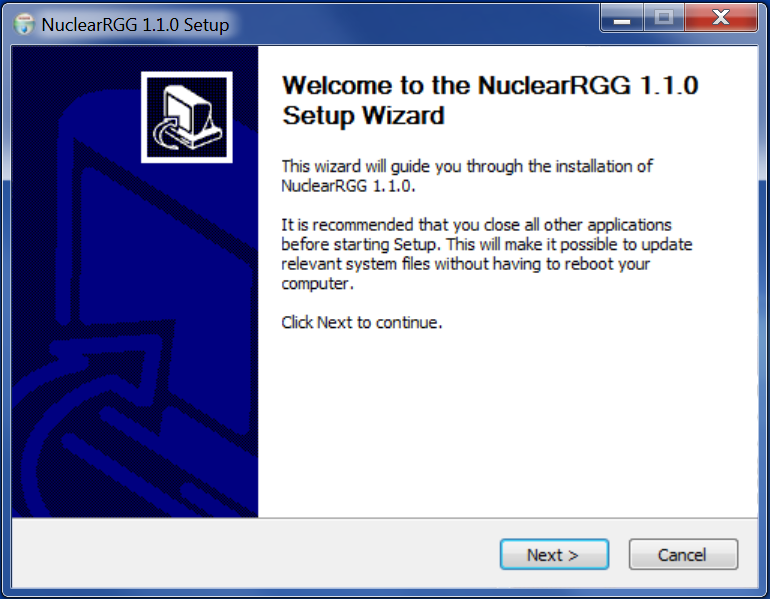
\includegraphics[width=0.5\linewidth]{Images/windows-install-1.png}
		\caption{Beginning the installation process.}
		\label{fig:WindowsInstall1}
	\end{center}
\end{figure}

Click \ui{Next}[Windows Installer] to continue and agree to the license displayed.  On the next screen (shown below), either use the default install location or select one of your own.  Click \ui{Next}[Windows Installer].

\begin{figure}[H]
	\begin{center}
		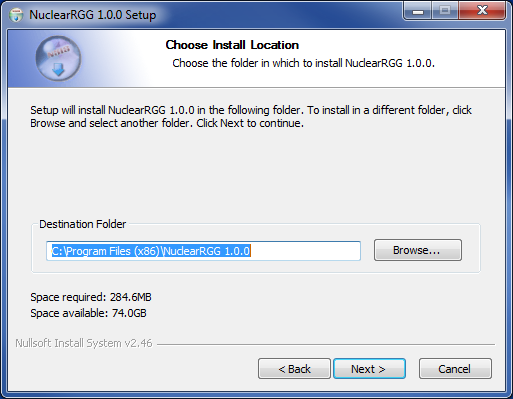
\includegraphics[width=0.5\linewidth]{Images/windows-install-2.png}
		\caption{Selecting the install location.}
		\label{fig:WindowsInstall2}
	\end{center}
\end{figure}

On the next window (shown below), select whether or not you'd like a Start Menu Folder to be created for RGG.  If you would not link a Start Menu Folder to be created, select the \ui{Do not create shortcuts box}[Windows Installer].  Otherwise, confirm the Start Menu Folder name you'd like to use.  Click install to have the installer extract the binaries.

\begin{figure}[H]
	\begin{center}
		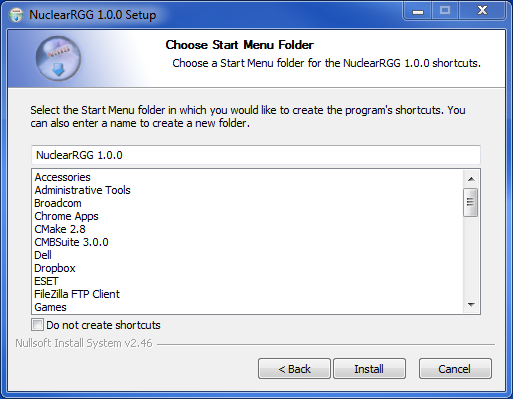
\includegraphics[width=0.5\linewidth]{Images/windows-install-3.png}
		\caption{Configuring Start Menu Folders.}
		\label{fig:WindowsInstall3}
	\end{center}
\end{figure}

A window should come up to confirm that RGG has been sucessfully installed on your computer.  At this point, you can click \ui{Finish}[Windows Installer] to close this wizard.

\section{Mac}
\toIndex{Mac Installation}
We use a standard drag and drop installer on Mac.  Simply mount the .dmg file and drag the RGG app into the Applications folder alias.

\section{Linux}
\toIndex{Linux Installation}
\todo{Figure out what CPack Generator we use for Linux packages.  Will we distribute a .deb, .rpm, or only tarballs and zip archives?}

\part{Using RGG}

\chapter{A Tour}
\label{chapter:ATour}
\section{Conceptual Overview And Terminology}

There are several concepts associated with RGG that must be understood before the user interface or workflow will seem sensible.

\subsection{Cores}
\toIndex{Cores}
The highest-level unit that RGG constructs is the core itself.  Cores can have either a rectilinear or hexagonal geometry to them.  This helps to define their lattice, or the grid on to which assemblies can be placed.  Cores are made up of assemblies arranged in a particular manner on the core lattice.  These cores can be translated into a mesh by MeshKit.

\subsection{Assemblies}
\toIndex{Assemblies}
As stated above, assemblies comprise cores.  Assemblies specify an arrangement of pins and ducts on their own lattice.  Think of assemblies as a configuration or specification of pins and ducts.

\subsection{Same As Assembly}
\toIndex{SameAsAssembly}
There are times where the user want to have an assembly with different material set and Neumann set start ids.  This is accomplished by a Same As Assembly, which links the desired assembly with the slightly different parameters.

\subsection{Pins}
\toIndex{Pins}
Pins are cylinders or frustums that model fuel pins, control rods, and the like.  They have a name, a label, a material or set of materials, and other diverse properties.

\subsection{Ducts}
\toIndex{Ducts}
Ducts are what surround the fuel pins -- in combination, they define the material composition of the space between pins in the lattice cells.

\subsection{Materials}
\toIndex{Materials}
Materials describe physical properties of a pin or duct.  Materials are assigned to pins and ducts in order to produce a mesh that can be used to accurately perform simulations.

\subsection{Meshes}
\toIndex{Meshes}
A mesh is a tetrahedral (triangular pyramid) or hexahedral (rectangular prism) representation of the core at a level of granularity sufficient for accurate simulation.  In RGG, they are produced by MeshKit.  This is the end product of RGG; the mesh is then fed into some other analytical software to perform the requested simulation.

Now that we've covered some high-level concepts, we're ready to look at an overview of the user interface.
\section{Basic User Interface Overview}
\subsection{Main Window Layout}
All user interaction takes place within the main window.  The main window is comprised of several movable widgets that can moved around or floating, depending on what best facilitates the work flow.  The main movable widgets are \ui{input}[input panel], \ui{properties panel},  \ui{3D view}, \ui{2D view}, and \ui{Mesh view}.  At start \ui{3D view}, \ui{2D view}, and \ui{Mesh view} are combined together in the visualization area, selectable by tab, but they can be moved.  There are two non-movable widgets.  The first non-movable widget is the \ui{toolbar}, located above the \ui{input}[input panel] and has icons for often used actions and the z-scaling controls.  The second non-movable widget is the \ui{menu}, located above the \ui{toolbar}. Refer to Figure \ref{fig:mainwindow1} to see these pictorally.

\begin{figure}[H]
	\begin{center}
		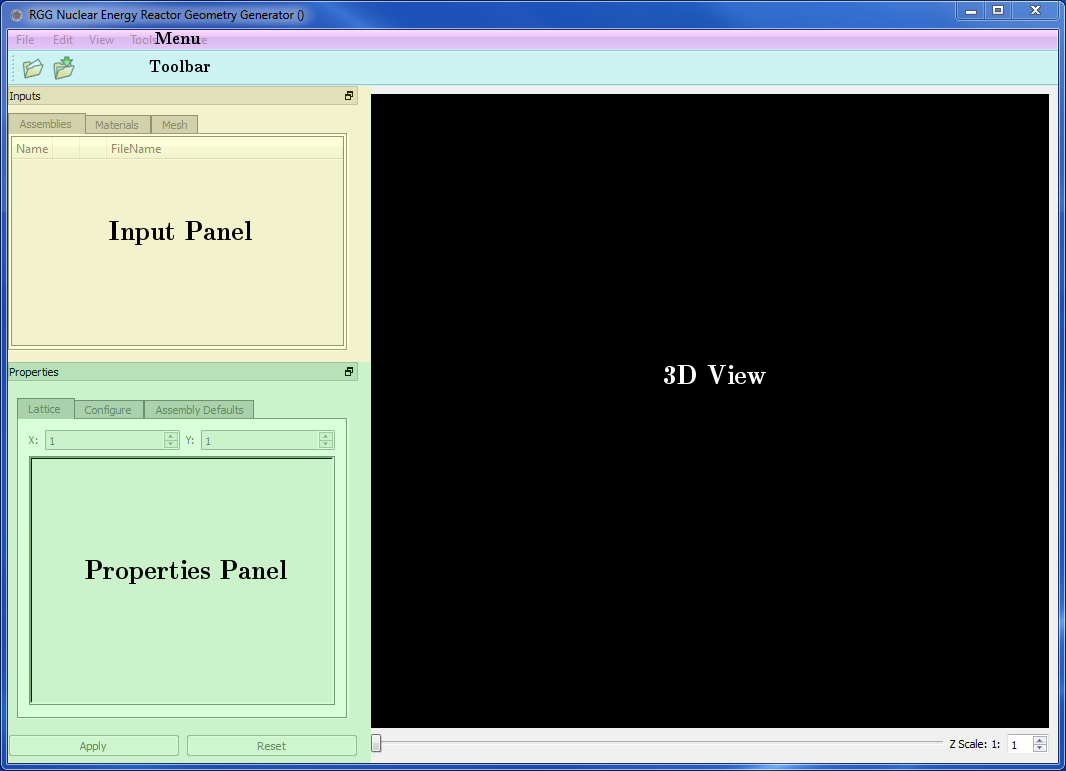
\includegraphics[width=\linewidth]{Images/main-window-layout.png}
		\caption{Layout of the \ui{main window}.}
		\label{fig:mainwindow1}
	\end{center}
\end{figure}


\subsection{Input Panel}
The \ui{input panel} has three tabs: the \ui{assemblies tab}, the \ui{materials tab}, and the \ui{mesh tab}.

\subsubsection{Assemblies Tab}
The \ui{assemblies tab} shows the hierarchal nature of the core, assemblies, pins and ducts.  Recall that a core is composed of assemblies which are placed in the core's lattice, and that these assemblies are in turn composed of pins and ducts that are placed in the assembly lattice.  When 

\begin{figure}[H]
	\begin{center}
		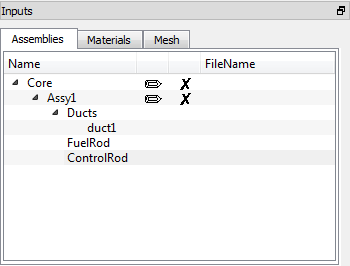
\includegraphics[width=0.5\linewidth]{Images/assemblies-tab.png}
		\caption{The assemblies tab shows the core, assembly, pin, and duct hierarchy.}
		\label{fig:mainwindow2}
	\end{center}
\end{figure}

Note you can check to see if the core or an assembly has had changes made to it since the last save.  A \ui{pencil icon} (as shown in Figure \ref{fig:mainwindow2}) indicates that edits have been made since the file was last saved.  A \ui{green box icon} indicates that the file is up to date.

You can also see the status of mesh files here.  An \ui{x icon} (as shown, to the right of the \ui{pencil icon}) indicates that mesh files have not been generated (or haven't been recreated since edits to the associated core or assembly), while \ui{green box icons} indicate that they are up to date.

\subsubsection{Materials Tab}
\toIndex{Materials}
The \ui{materials tab} (Figure ~\ref{fig:mainwindow3}) details the list of available materials, their associated colors, and whether or not they are viewable.  You can use this tab to create, remove, import, and export materials, as well as edit the labels and colors of materials and toggle whether or not they are shown in the \ui{3D view} or \ui{Mesh view}.  You can also filter the list based on materials used in the core or currently displayed in either the \ui{3D view} or \ui{Mesh view}.

\begin{figure}[h]
	\begin{center}
		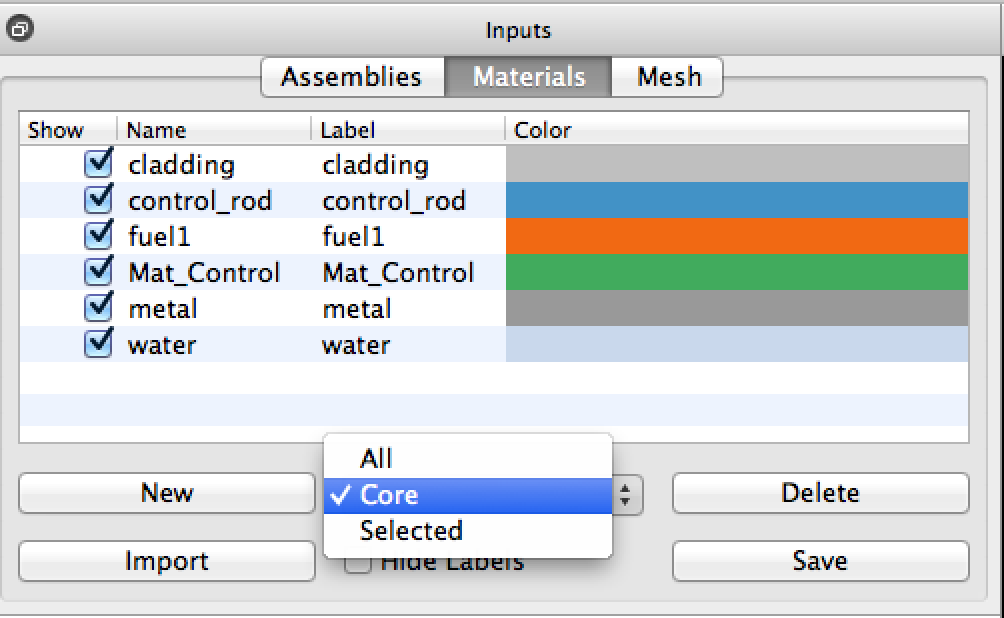
\includegraphics[width=0.5\linewidth]{Images/materials-tab.png}
		\caption{The materials tab shows available materials.}
		\label{fig:mainwindow3}
	\end{center}
\end{figure}

\subsubsection{Mesh Tab}
The \ui{mesh tab} (Figure ~\ref{fig:mainwindow4}) allows you to control the viewing of the mesh.  It is only available when a mesh is loaded.  It has the options to control what shows up in the \ui{Mesh view}, including the ability to show volumes, boundaries, surfaces, Neumann sets, Dirichlet sets, Material sets, show mesh edges, and to colorize the different volumes.  More information on this tab is given in Section \ref{section:DisplayingMeshes}.

\begin{figure}[h]
	\begin{center}
		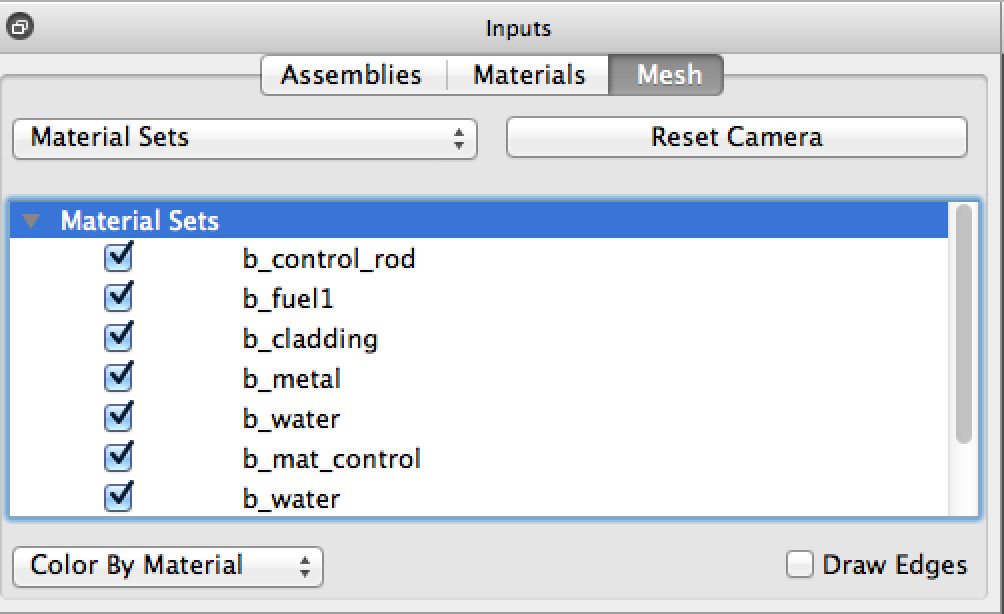
\includegraphics[width=0.5\linewidth]{Images/mash-tab.png}
		\caption{Used to control the mesh}
		\label{fig:mainwindow4}
	\end{center}
\end{figure}

\subsection{Properties Panel}
The \ui{properties panel} changes depending on the current state of the input panel's \ui{assemblies tab}.

\begin{itemize}
	\item{If you're clicking on a core, it will display three tabs: the \ui{lattice tab}, the \ui{configure tab}, and the \ui{assembly defaults tab}.}
	\item{If you're clicking on an assembly, it will display the \ui{lattice tab} and \ui{configure tab}.  Note that the assembly has a different \ui{lattice tab} and \ui{configure tab} from the core.}
	\item{If you're clicking on a duct, it will display the \ui{duct tab}.}
	\item{If you're clicking on a pin, it will display the \ui{pin tab}.}
\end{itemize}

\subsubsection{Lattice Tab}
The \ui{lattice tab} controls the number of layers (in a hexagonal core) or the dimensions (in a rectilinear core) to get the desired lattice geometry.  For cores, it also controls the \ui{Reactor Vessel} and \ui{Boundary Layer}s.  For assemblies, there is a checkbox to allow for auto-centering the pins.  Also for assemblies, this tab controls the \ui{2D view} color and label.  There is also controls for assembly rotation and the \ui{duct} used.  See Figure \ref{fig:latticetab}.

\begin{figure}
\centering
\begin{subfigure}{.5\textwidth}
  \centering
  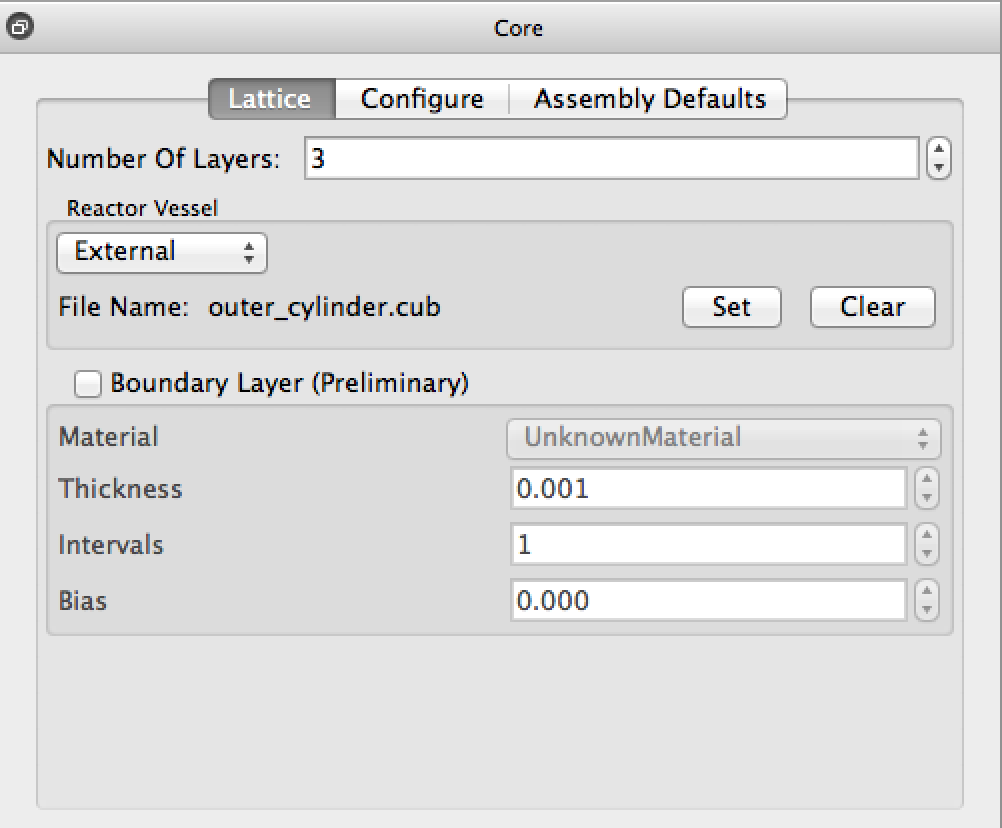
\includegraphics[width=0.6\linewidth]{Images/core-lattice.png}
  \caption{Core Lattice Tab.}
  \label{fig:rectSetMaterial}
\end{subfigure}%
\begin{subfigure}{.5\textwidth}
  \centering
  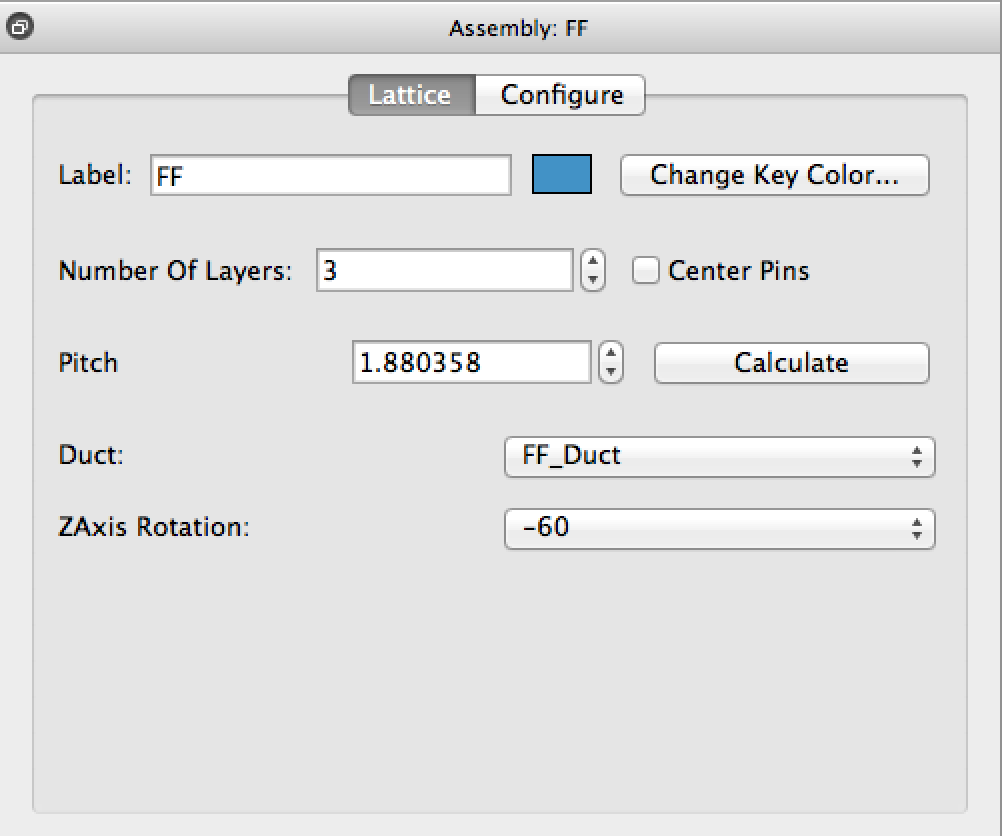
\includegraphics[width=0.6\linewidth]{Images/assy-lattice.png}
  \caption{The Assembly Lattice Tab.}
  \label{fig:rectDuctResult}
\end{subfigure}
\caption{The two versions of the Lattice Tab.}
\label{fig:latticetab}
\end{figure}


\subsubsection{Configure Tab}
This tab allows you to customize other meshing parameters from MeshKit files which are not currently provided an interface in the GUI. See Chapter \ref{chapter:Meshing} for information on how to mesh your core.

\subsubsection{Assembly Defaults Tab}
The \ui{assembly defaults tab} allows you to specify general meshing information.  You can set whether the mesh you want to generate will be tetrahedral or hexahedral, and also change the default dimensions of the ducts comprising your core.  Changing these values will propagate all the way down to every component, so you can change it all in one place instead of adjusting the height of every duct in every assembly.

\subsubsection{Duct Tab}
The \ui{duct tab} exposes the different configuration options for a duct piece.  You can change the position and dimensional settings towards the top, the duct pitch, and the duct material (with associated normalized thickness, if desired).

\subsubsection{Pin Tab}
The \ui{pin tab} allows you to change the key color of the pin, specify the pin material(s), and create, remove, or edit pin pieces.

\subsection{3D View}
The \ui{3D view} (Figure ~\ref{fig:3DView}) displays a representation of the current component.  You can use the following controls to interact with it:

\begin{itemize}
	\item{To rotate, click with the left mouse button.}
	\item{To pan, either shift-click with the left mouse button or use the middle mouse button.}
	\item{To zoom, click with the right mouse button.}
\end{itemize}

\begin{figure}[h]
	\begin{center}
		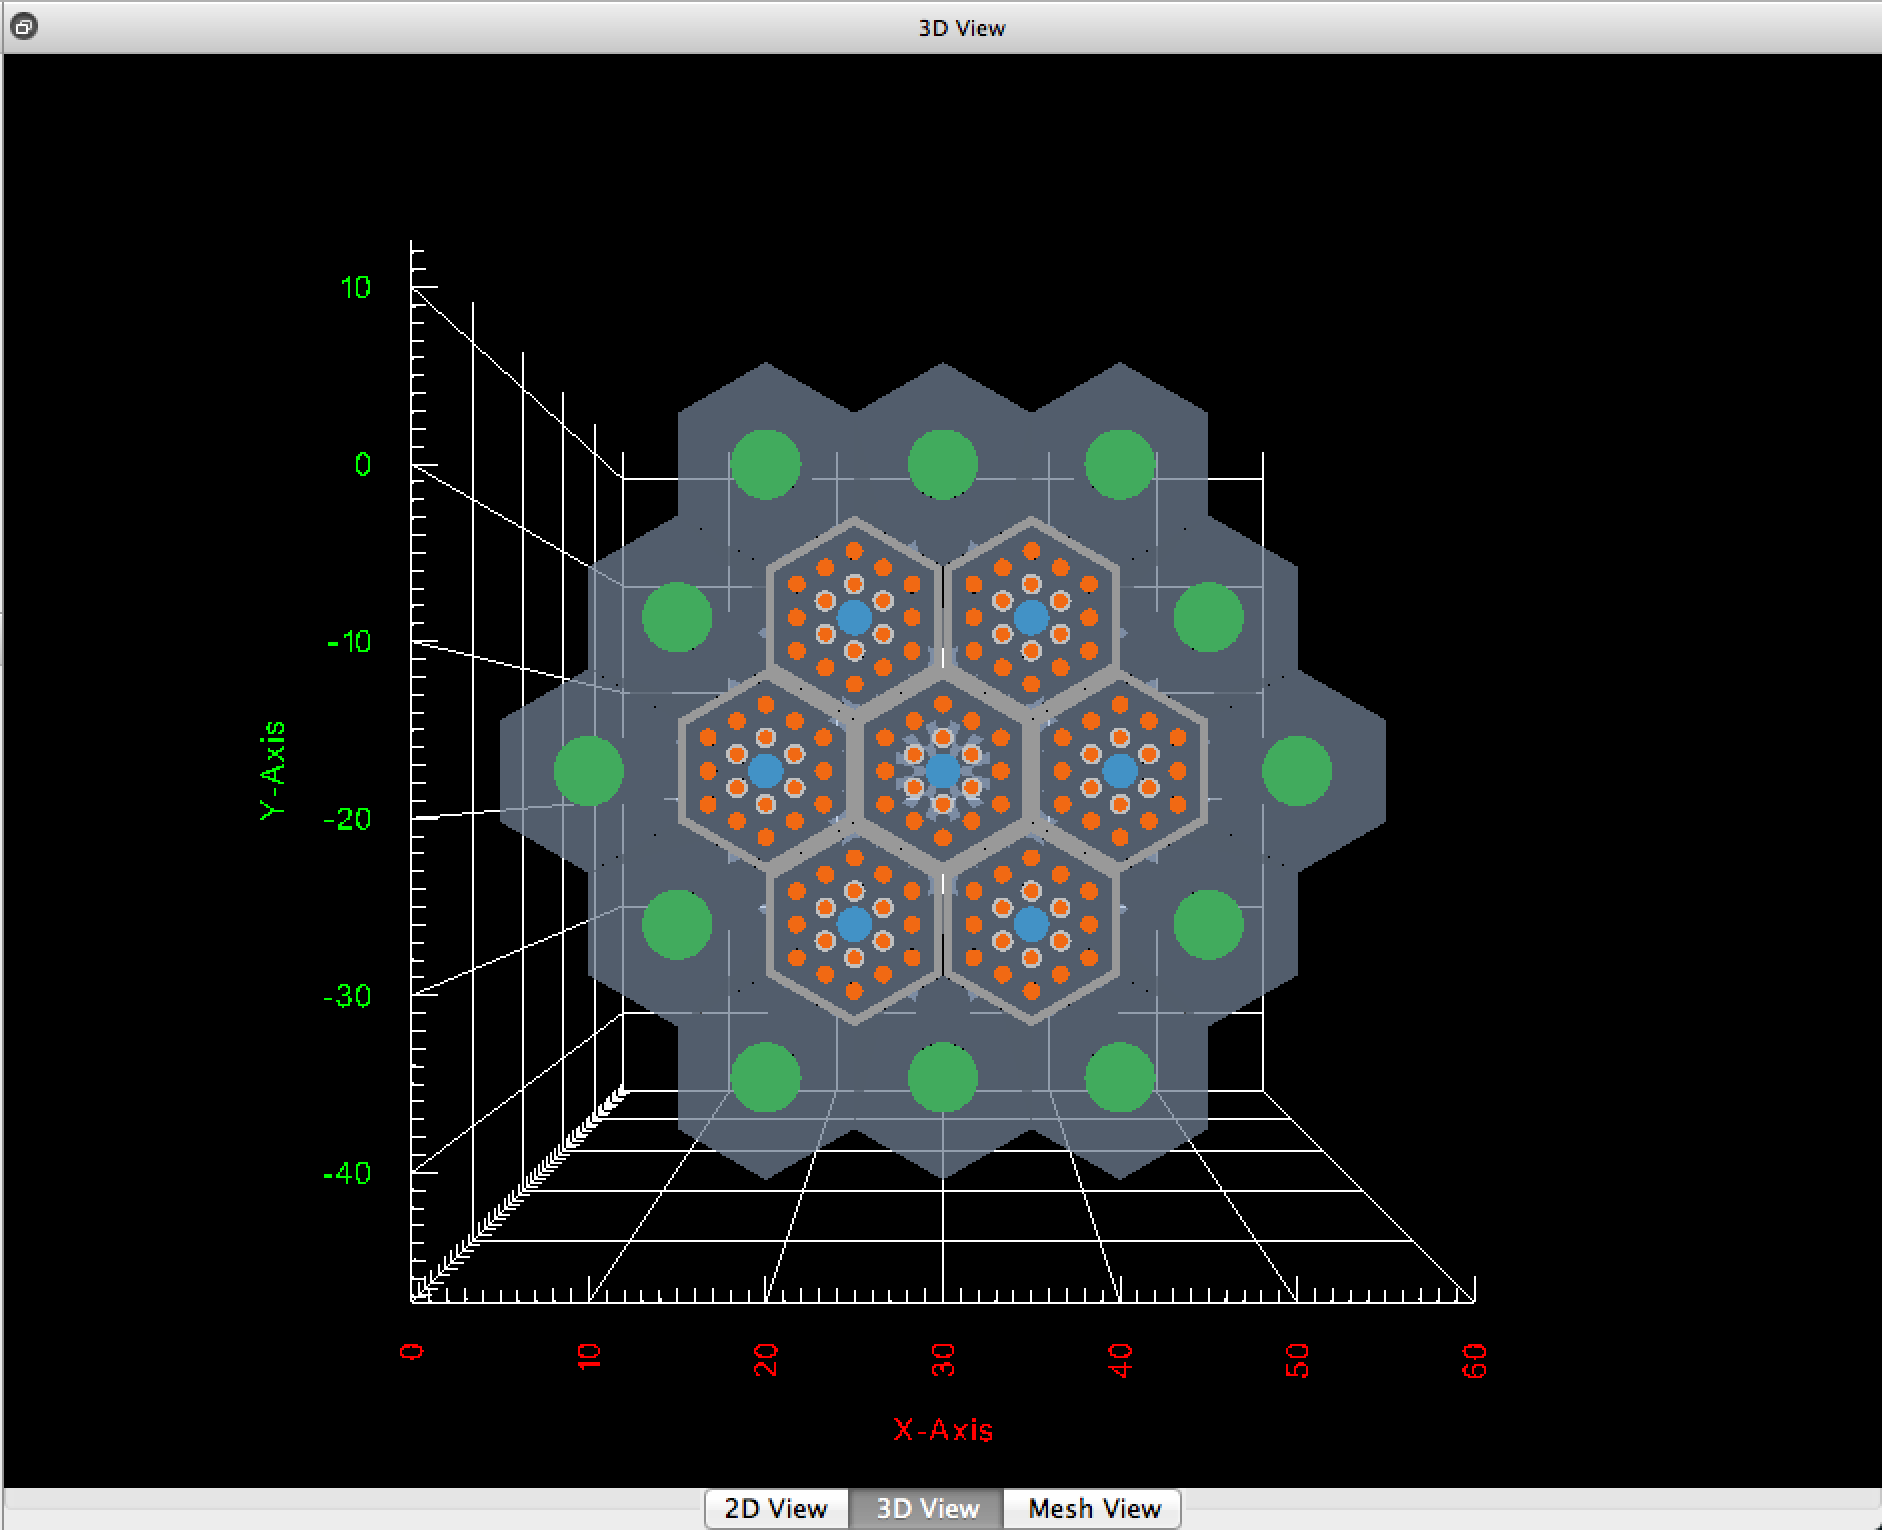
\includegraphics[width=0.5\linewidth]{Images/3DView.png}
		\caption{The 3D View}
		\label{fig:3DView}
	\end{center}
\end{figure}

Similar to the \ui{properties panel}, the \ui{3D view} changes depending on what is selected in the assemblies tab of the input panel.

\begin{itemize}
	\item{If you're clicking on a core, it will display the entire core.}
	\item{If you're clicking on an assembly or a duct, it will display the assembly.}
	\item{If you're clicking on a pin, it will display the pin.}
\end{itemize}

\subsection{2D View}
The \ui{2D view} (Figure ~\ref{fig:2DView}) provides a 2d schematic of the core or assembly depending which is selected. Each assembly or pin represented here will be filled with its corresponding key color.

You can edit this information by moving you mouse over the cell you want to edit and then right-click on each cell to select the desired assembly or pin.  In the pop-up menu, there are options to \ui{Replace All With} and \ui{Fill Ring With}. \ui{Replace All With} replaces every cell that is same component with the desired assembly or pin.  \ui{Fill Ring With} fills every cell in the ring with the desired assembly or pin.  Alternatively, you can drag and drop an existing component onto the cell.

\begin{figure}[h]
	\begin{center}
		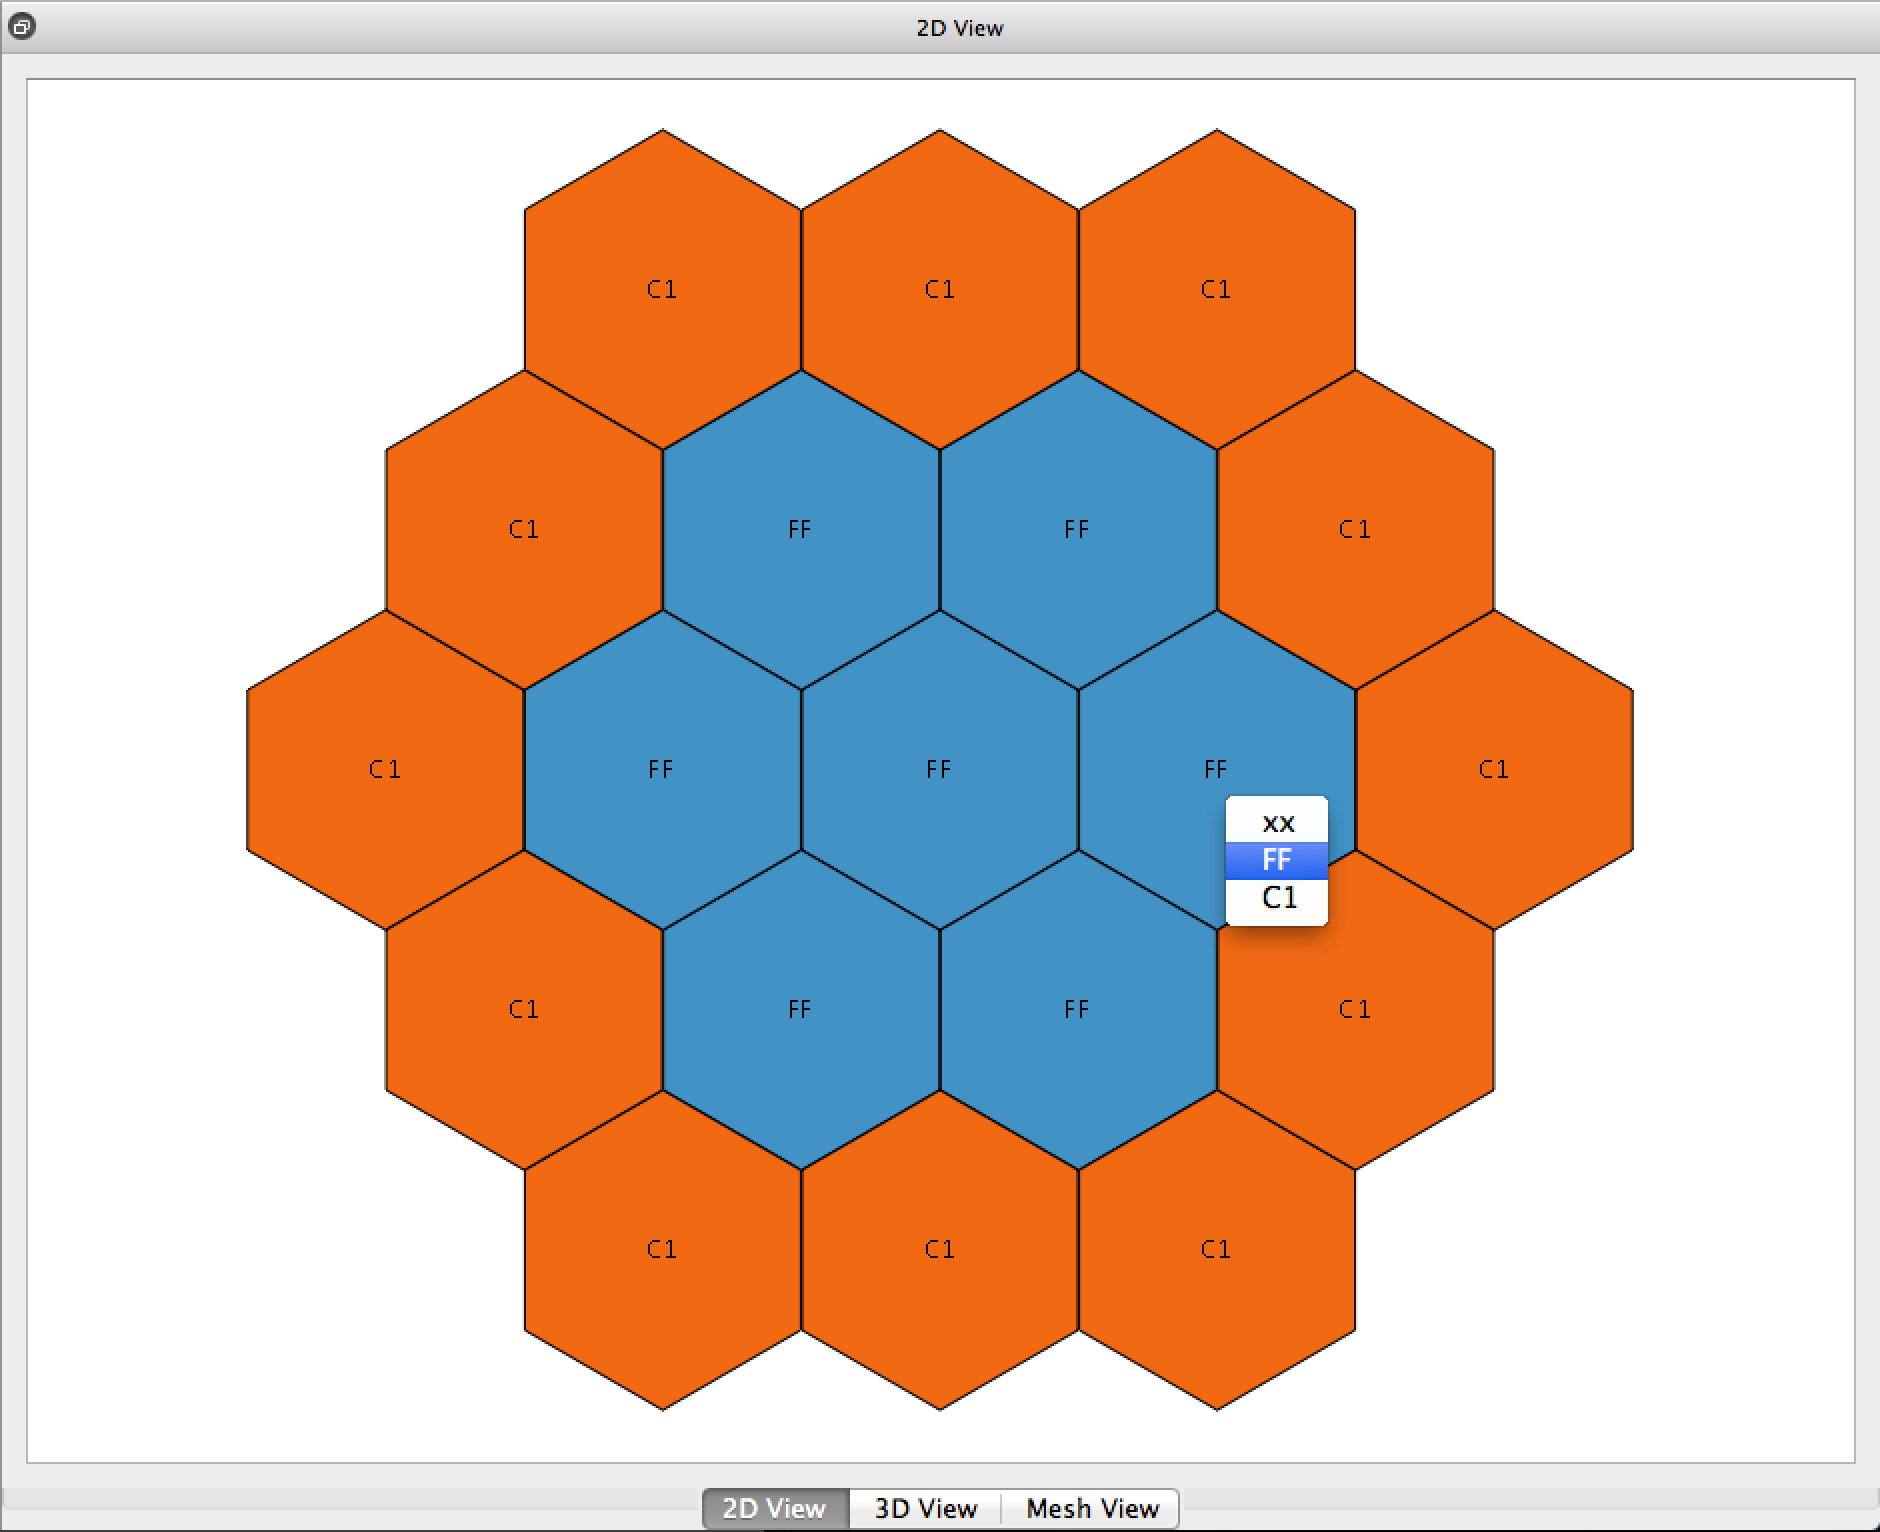
\includegraphics[width=0.5\linewidth]{Images/2DView.png}
		\caption{The 2D View}
		\label{fig:2DView}
	\end{center}
\end{figure}

\subsection{Mesh View}
The \ui{Mesh view} (Figure ~\ref{fig:MeshView}) is only visible if a mesh has been loaded.  The Mesh Tab controls what is displayed here.

\begin{figure}[h]
	\begin{center}
		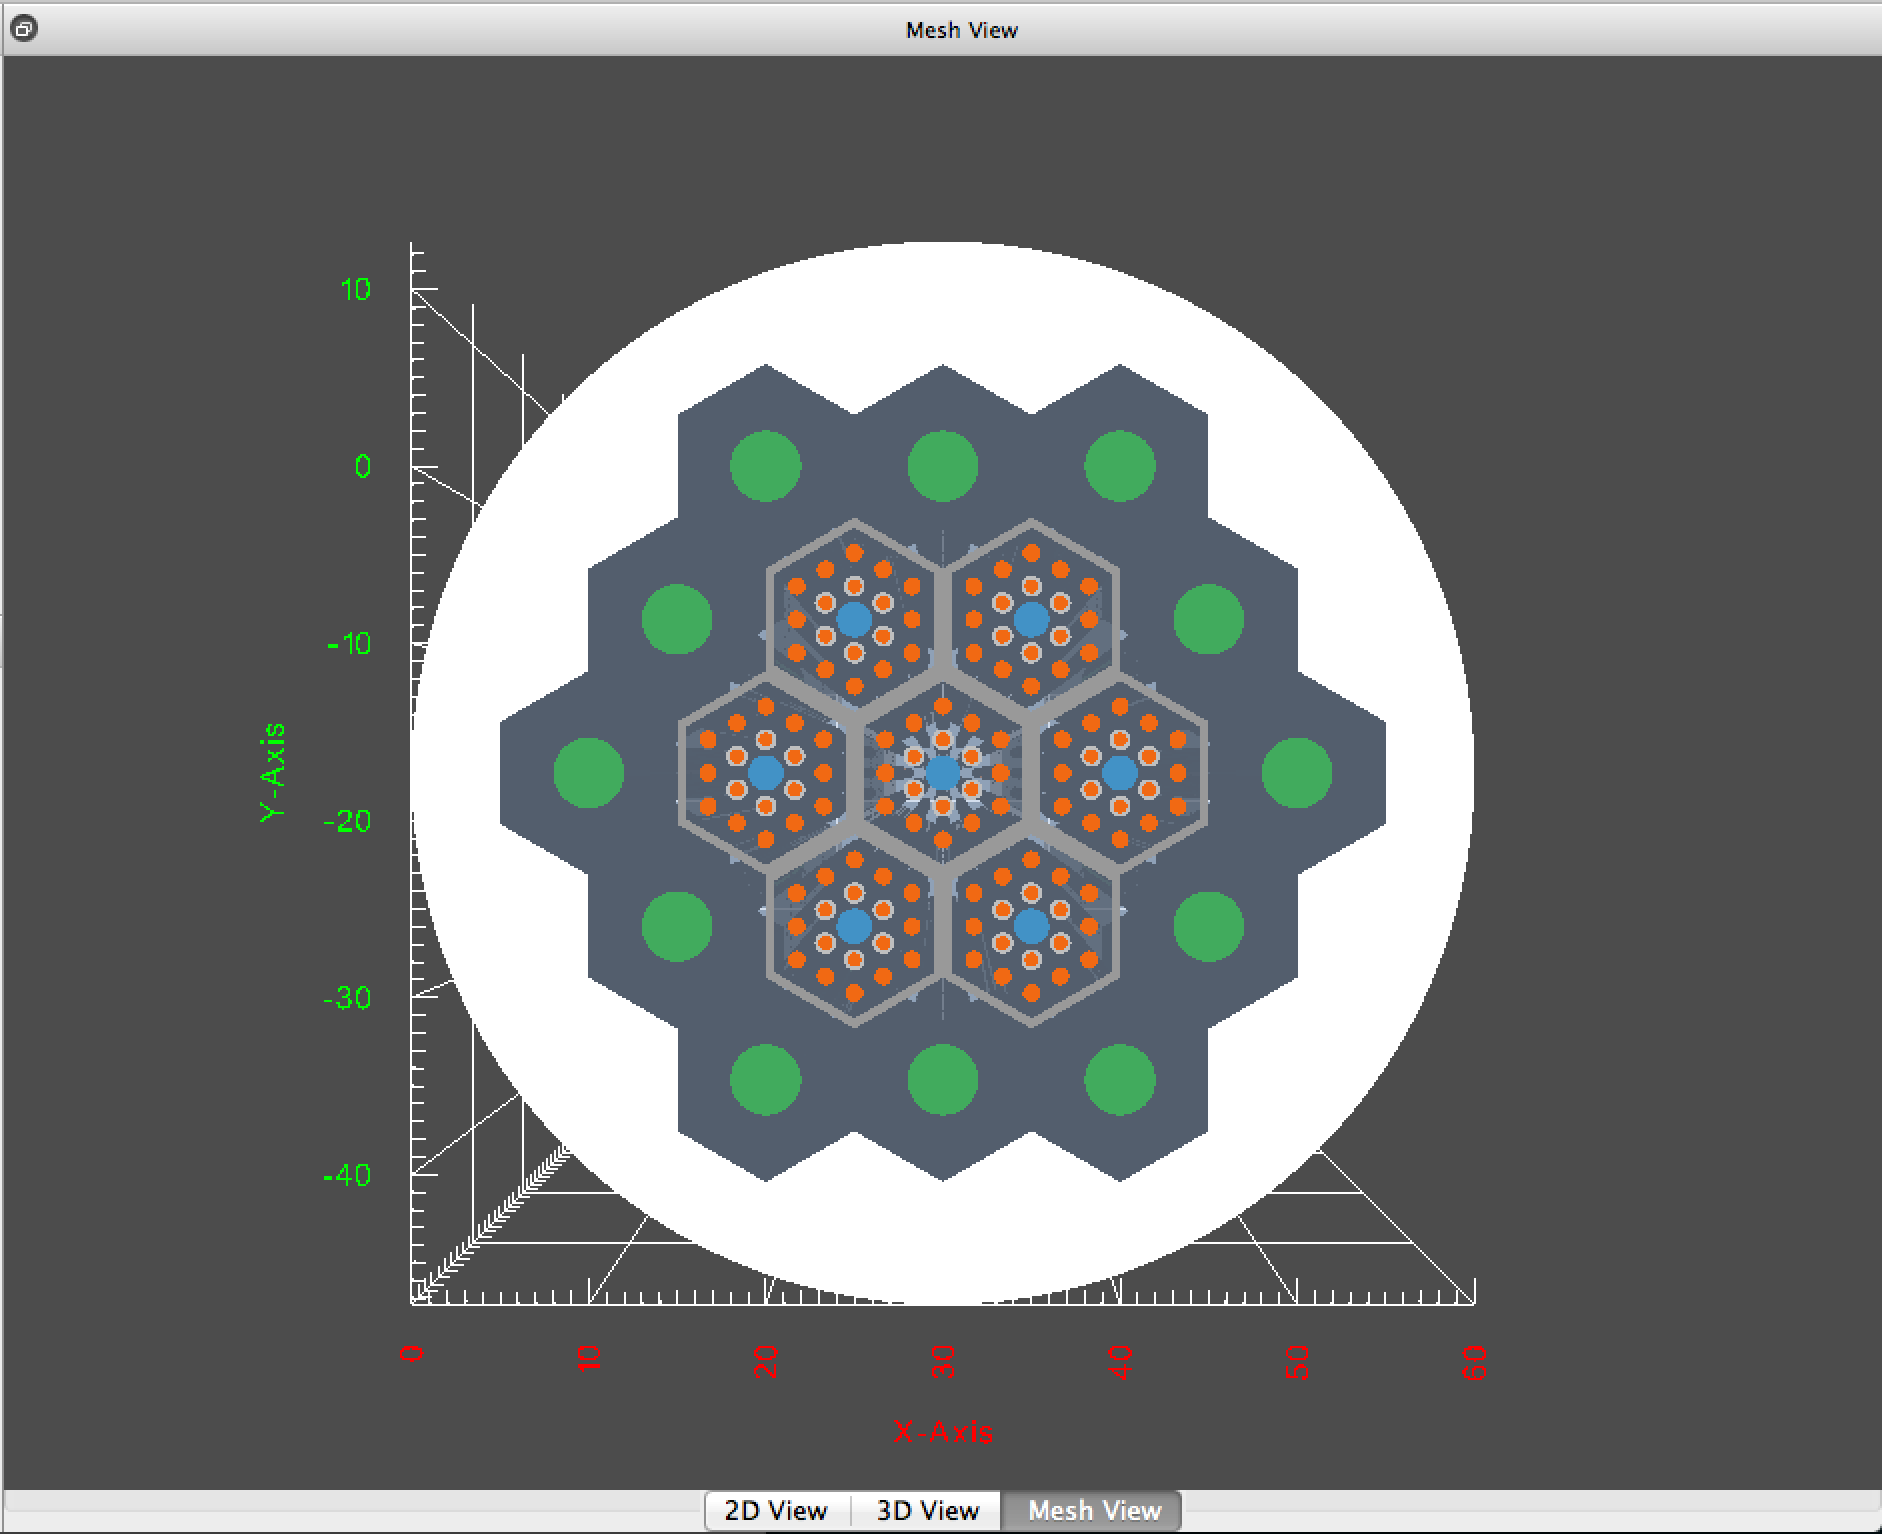
\includegraphics[width=0.5\linewidth]{Images/MeshView.png}
		\caption{The Mesh View}
		\label{fig:MeshView}
	\end{center}
\end{figure}



\chapter{Meshing}
\label{chapter:Meshing}
Nunc viverra varius odio, at pharetra velit laoreet nec. Donec sagittis vestibulum erat posuere auctor. Ut at interdum tortor, volutpat ullamcorper massa. Vestibulum a tempus quam, sed fringilla nibh. Nam semper est a ante venenatis, non bibendum lectus auctor. Duis blandit lacus urna, eget dictum sem pretium eget. Etiam bibendum semper placerat. Pellentesque commodo eros tempor justo congue, vel aliquam quam tristique. Donec eu magna ornare nisl vulputate pretium. Pellentesque at orci et velit luctus elementum eu eget dui. In hac habitasse platea dictumst.
\section{Generating a Mesh}

Now that the system preferences have been adjusted to include AssyGen, Cubit, and CoreGen, you can generate a mesh  though the \ui{Run MeshKit RGG dialog} accessed through the \ui{tools menu}.  Note the ``x" icon in the third column of the assemblies and core in the \ui{inputs panel}.  This designates that RGG believes that these components need to be meshed.

\begin{figure}[H]
	\begin{center}
		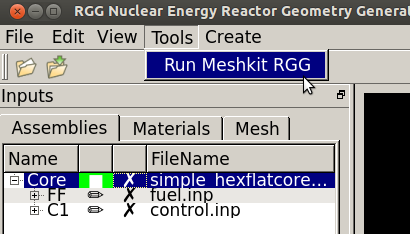
\includegraphics[width=0.5\linewidth]{Images/mesh-3.png}
		\caption{Opening the Run MeshKit RGG dialog.  The \ui{x icon}s denote that the FF and C1 assemblies need to be meshed.}
		\label{fig:Mesh3}
	\end{center}
\end{figure}

You will be prompted to save changes before proceeding if what is loaded into RGG differs from its file on disk.

The dialog should be populated with the assemblies that need to be re-meshed automatically.  In the example below, two assemblies need to be meshed, which also means that the core must be remeshed.  If ``Keep Going on Error" is checked, RGG will process every possible Assembly Files after an error occurs.  Any job that depends on the erred job will not be run.  If it is not checked, RGG will quite processing after the first error.  Checking ``Keep Going on Error" is advised if there are a large number of files to be processed.

\begin{figure}[H]
	\begin{center}
		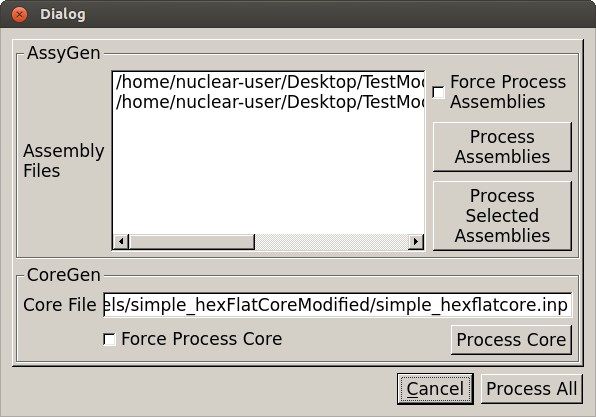
\includegraphics[width=0.5\linewidth]{Images/mesh-4.png}
		\caption{The Run MeshKit RGG dialog.}
		\label{fig:Mesh4}
	\end{center}
\end{figure}

One can force the generation of meshes regardless of their current state by using the \ui{force process assemblies checkbox} and the \ui{force process core checkbox} for an assembly or core, respectively.  To mesh both the core and assemblies, check both boxes and use the \ui{process all button}.  This is useful in cases where the exporting executables have changed.  A window that gives you the status of the processing should come up, similar to the shown in Figure \ref{fig:Mesh5}:

\begin{figure}[H]
	\begin{center}
		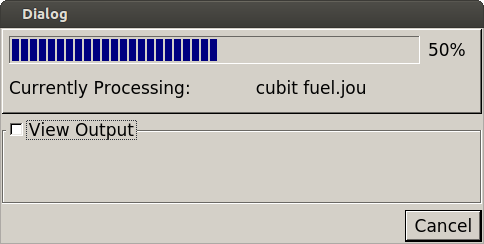
\includegraphics[width=0.5\linewidth]{Images/mesh-5.png}
		\caption{Running meshing.}
		\label{fig:Mesh5}
	\end{center}
\end{figure}

You can see the output of AssyGen, CoreGen, and Cubit by clicking on the \ui{view output checkbox}.  To cancel the current export, click the \ui{cancel button}.

To verify that the assemblies and core have been meshed, confirm that the \ui{x icon}s seen previously are now \ui{green square icon}s, as shown in Figure \ref{fig:Mesh6}.

\begin{figure}[H]
	\begin{center}
		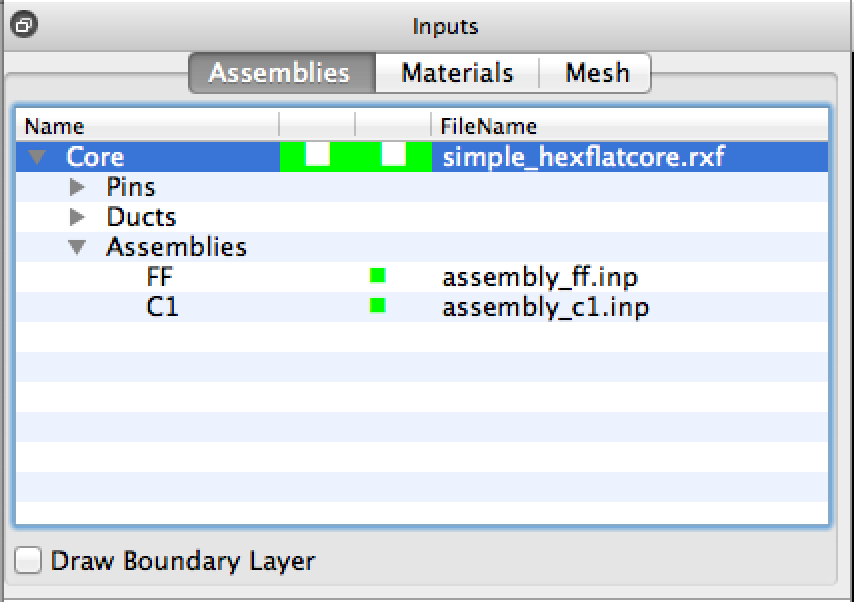
\includegraphics[width=0.5\linewidth]{Images/mesh-6.png}
		\caption{Verifying successful meshing.}
		\label{fig:Mesh6}
	\end{center}
\end{figure}

Note that the mesh needs to be loaded in after MeshKit creates it.  During this process, the tools menu is inaccessible.
\section{Displaying the Mesh}
\label{section:DisplayingMeshes}

Upon successful creation of a mesh, you either need to load it in manually via the \emph{open MOAB file dialog} accessed from the \emph{open MOAB file item} in the \emph{file menu}, or, if you've just meshed an INP file you lodaed in, the mesh will load in automatically.

\subsection{Views of the Mesh}
To control viewing the mesh, be sure to click on the \emph{mesh tab} of the \emph{inputs panel}.  RGG allows you to six different options to control the \emph{3D view} of the mesh, listed below:

\begin{itemize}
	\item{Volumes}
	\item{Boundary}
	\item{Surfaces}
	\item{Neumann Sets}
	\item{Dirichlet Sets}
	\item{Material Sets}
\end{itemize}

More detail on these views is provided below.  Additionally, you can check the \emph{show edges checkbox} to view the mesh superimposed on the 3D view and check the \emph{color checkbox} to colorize the different pieces of the view based on the option you've selected.

\subsubsection{Volumes}
Clicking the \emph{volumes option} shows all the volumes of the mesh.  Checking the color checkbox will colorize all of the distinct volumes in different colors.

\subsubsection{Boundary}
In this mode, RGG displays only the boundary conditions.  Checking the color checkbox will colorize all of the distinct volumes in different colors.

\subsubsection{Surfaces}
When the \emph{surfaces option} is selected, RGG displays only the surfaces of the mesh.

\subsubsection{Neumann Sets}
Clicking the \emph{Neumann Sets option} will show the natural boundary conditions on sides of domains.

\subsubsection{Dirichlet Sets}
Clicking the \emph{Dirichlet Sets option} will show the essential boundary conditions on points of domains.

\subsubsection{Material Sets}
Material sets displays all the volumes of the mesh, but colorizes them on a per material basis.  Additionally, you can toggle the visability of materials by checking and unchecking them in the \emph{materials tab} of the inputs panel.

\chapter{Advanced Techniques}
\label{chapter:AdvancedTechniques}

\chapter{Building Rectangular Cores}
\label{chapter:ExampleBuildingARectangularCore}
\subsection{Creating an Assembly Duct Composed of Water}

First, create a new rectilinear core, and add a new duct to the assembly by following ~\ref{fig:Rect1}.

\begin{figure}[htb]
\begin{center}
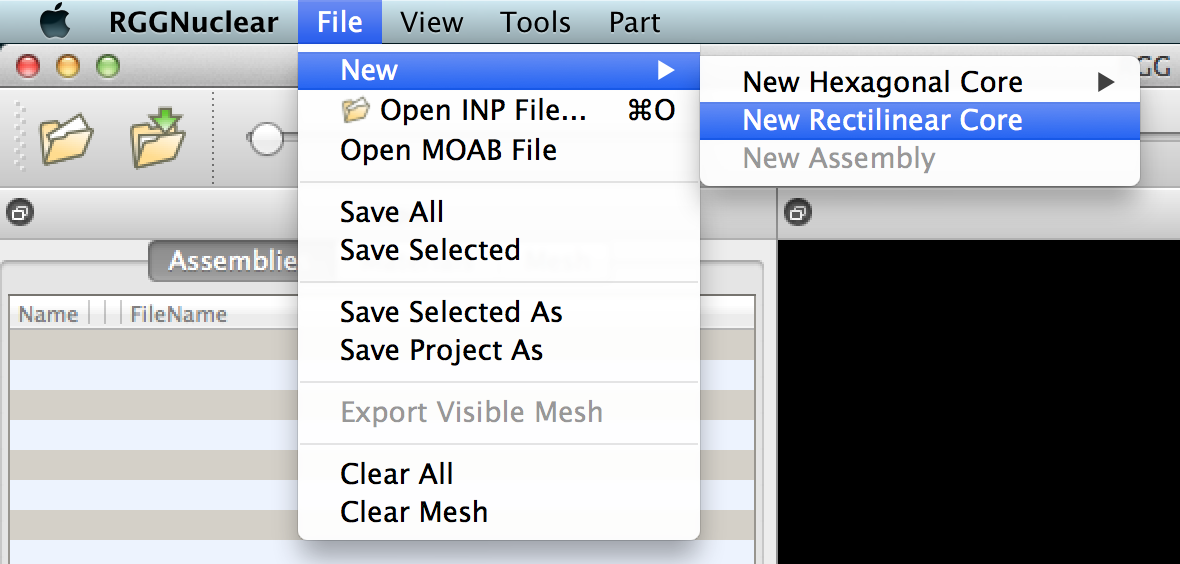
\includegraphics[width=0.5\linewidth]{Images/rect-1e1.png}
\caption{Select the option to create a new rectilinear assembly duct.}
\label{fig:Rect1}
\end{center}
\end{figure}

This results in a core with a single assembly with a duct of unknown material shown in ~\ref{fig:NewRect}.

\begin{figure}[htb]
\begin{center}
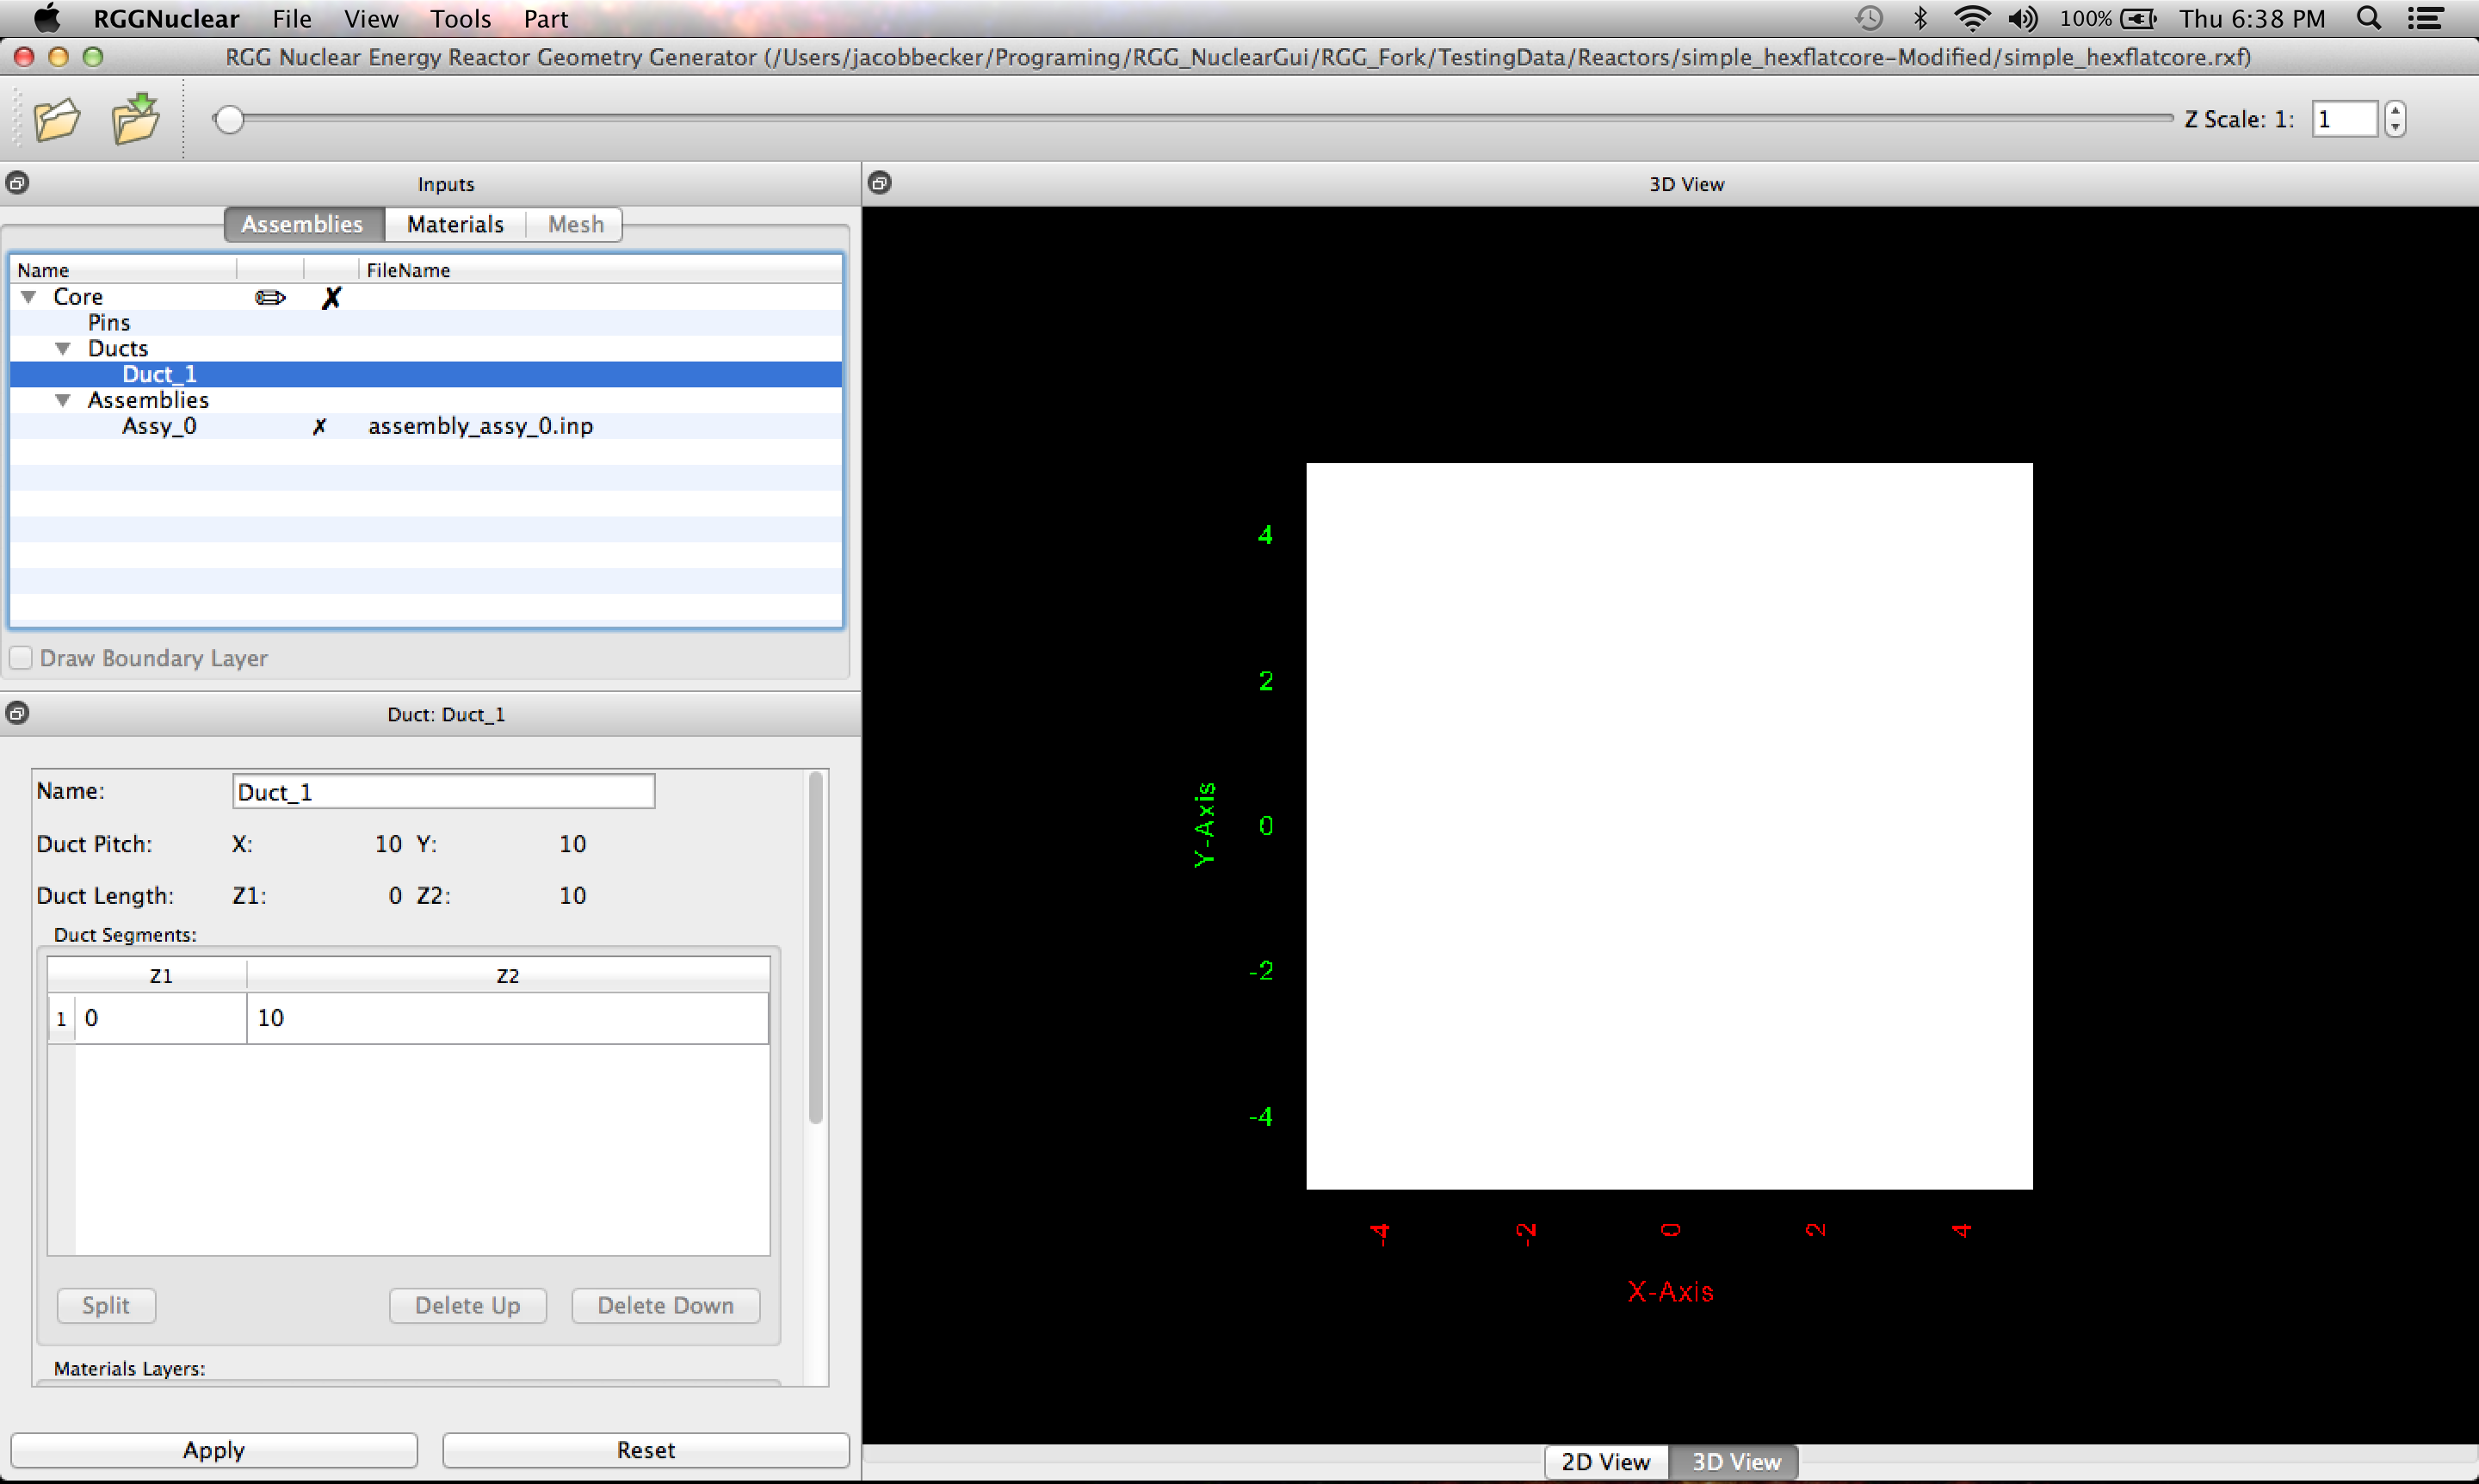
\includegraphics[width=0.5\linewidth]{Images/rect-init-model.png}
\caption{The initial rectangular core.}
\label{fig:NewRect}
\end{center}
\end{figure}

Now, to adjust the size of the duct, select the "Assembly Defaults" tab in Core's Properties Panel.  In this example, we are going to set the "Duct Thickness" to 15 (~\ref{fig:SetRectDuctDem}).

\begin{figure}[htb]
\begin{center}
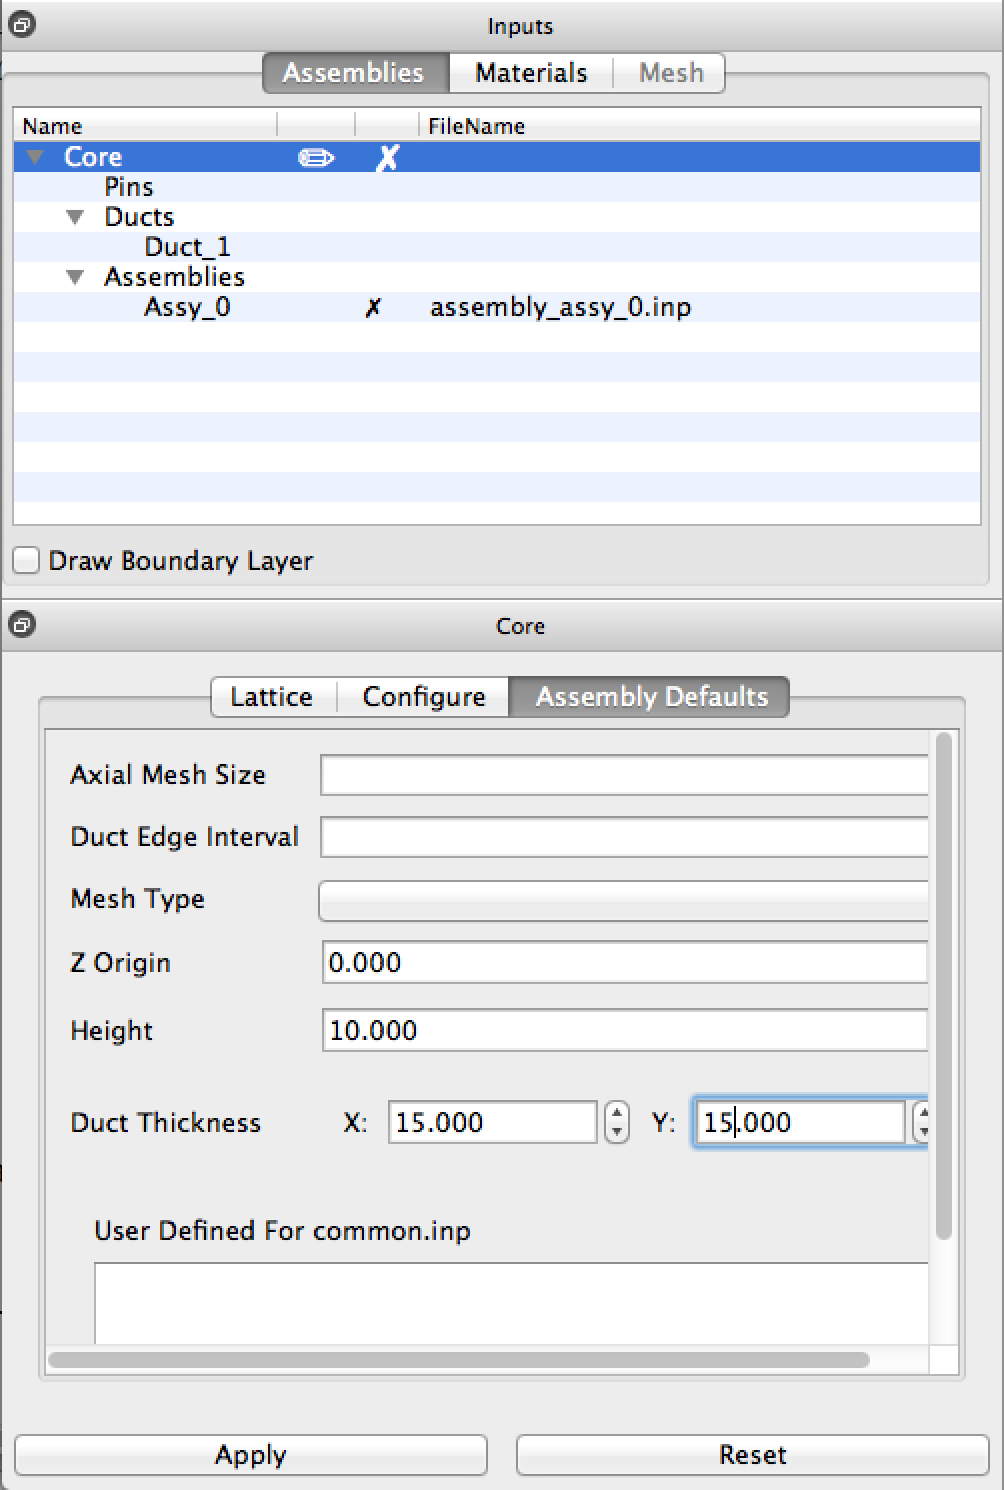
\includegraphics[width=0.5\linewidth]{Images/rect-set-dim.png}
\caption{The initial rectangular core.}
\label{fig:SetRectDuctDem}
\end{center}
\end{figure}

Next adjust the material of the Duct.  In the Inputs Panel, select the Duct.  Then, in the Duct's Properties Panel, select the first Duct Segment.  This populates Material Layers with the Duct Segments materials.  Now, select water in the material drop down box drop (~\ref{fig:rectSetMaterial}).  Then press Apply.  The result should look like ~\ref{fig:rectDuctResult}.

\begin{figure}
\centering
\begin{subfigure}{.5\textwidth}
  \centering
  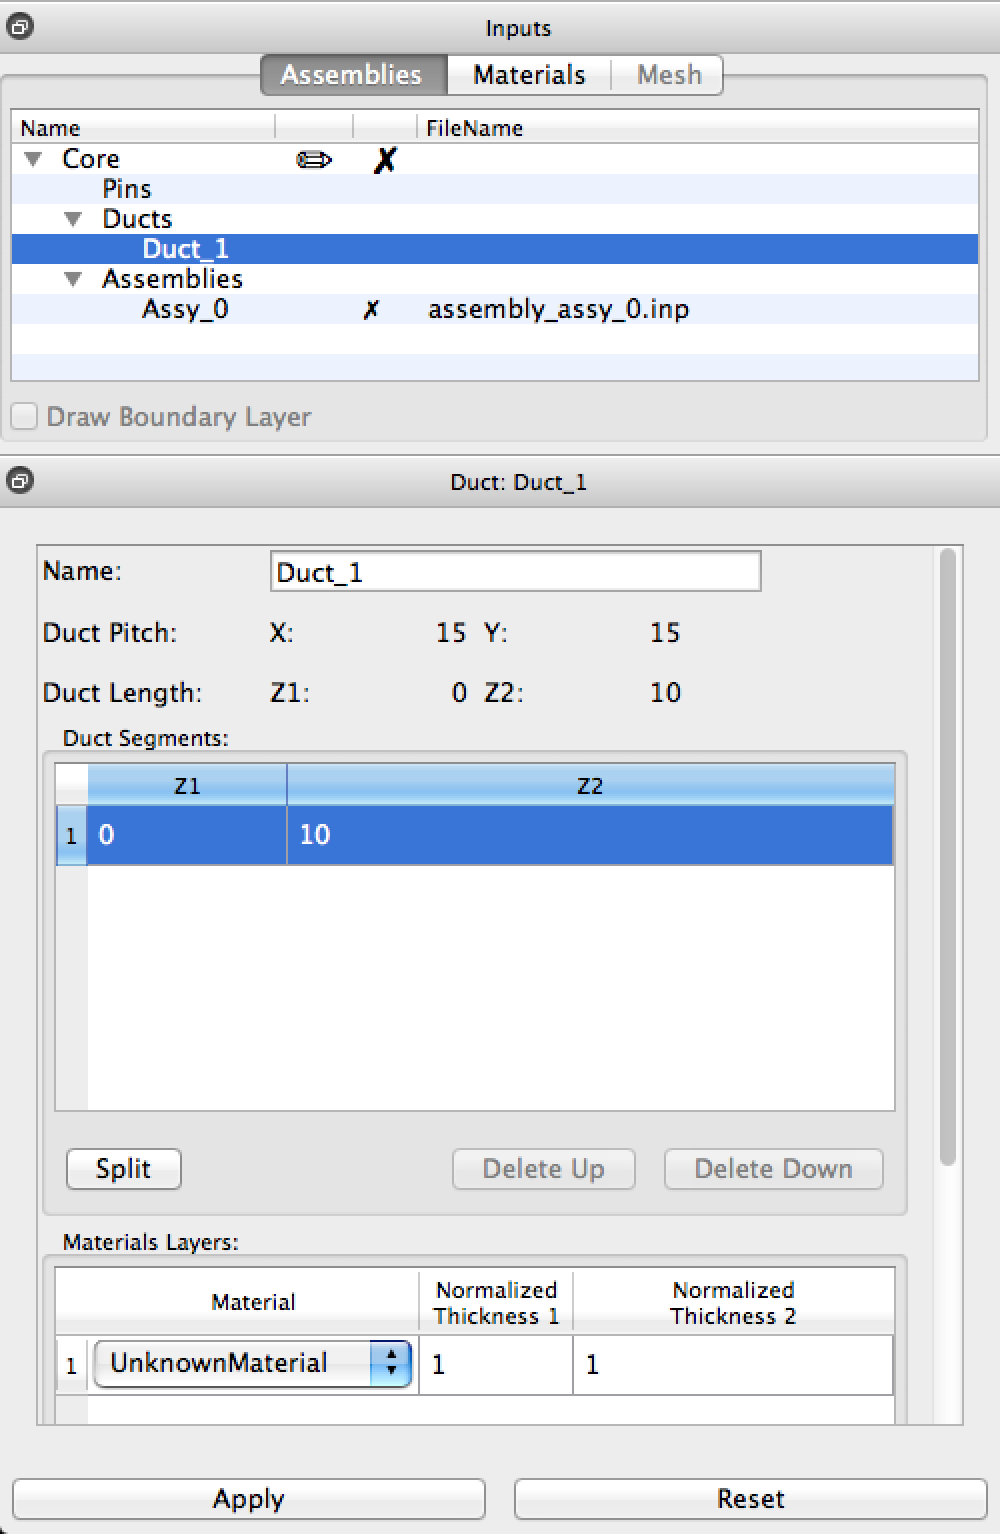
\includegraphics[width=0.7\linewidth]{Images/rect-set-material.png}
  \caption{Setting material of the duct.}
  \label{fig:rectSetMaterial}
\end{subfigure}%
\begin{subfigure}{.5\textwidth}
  \centering
  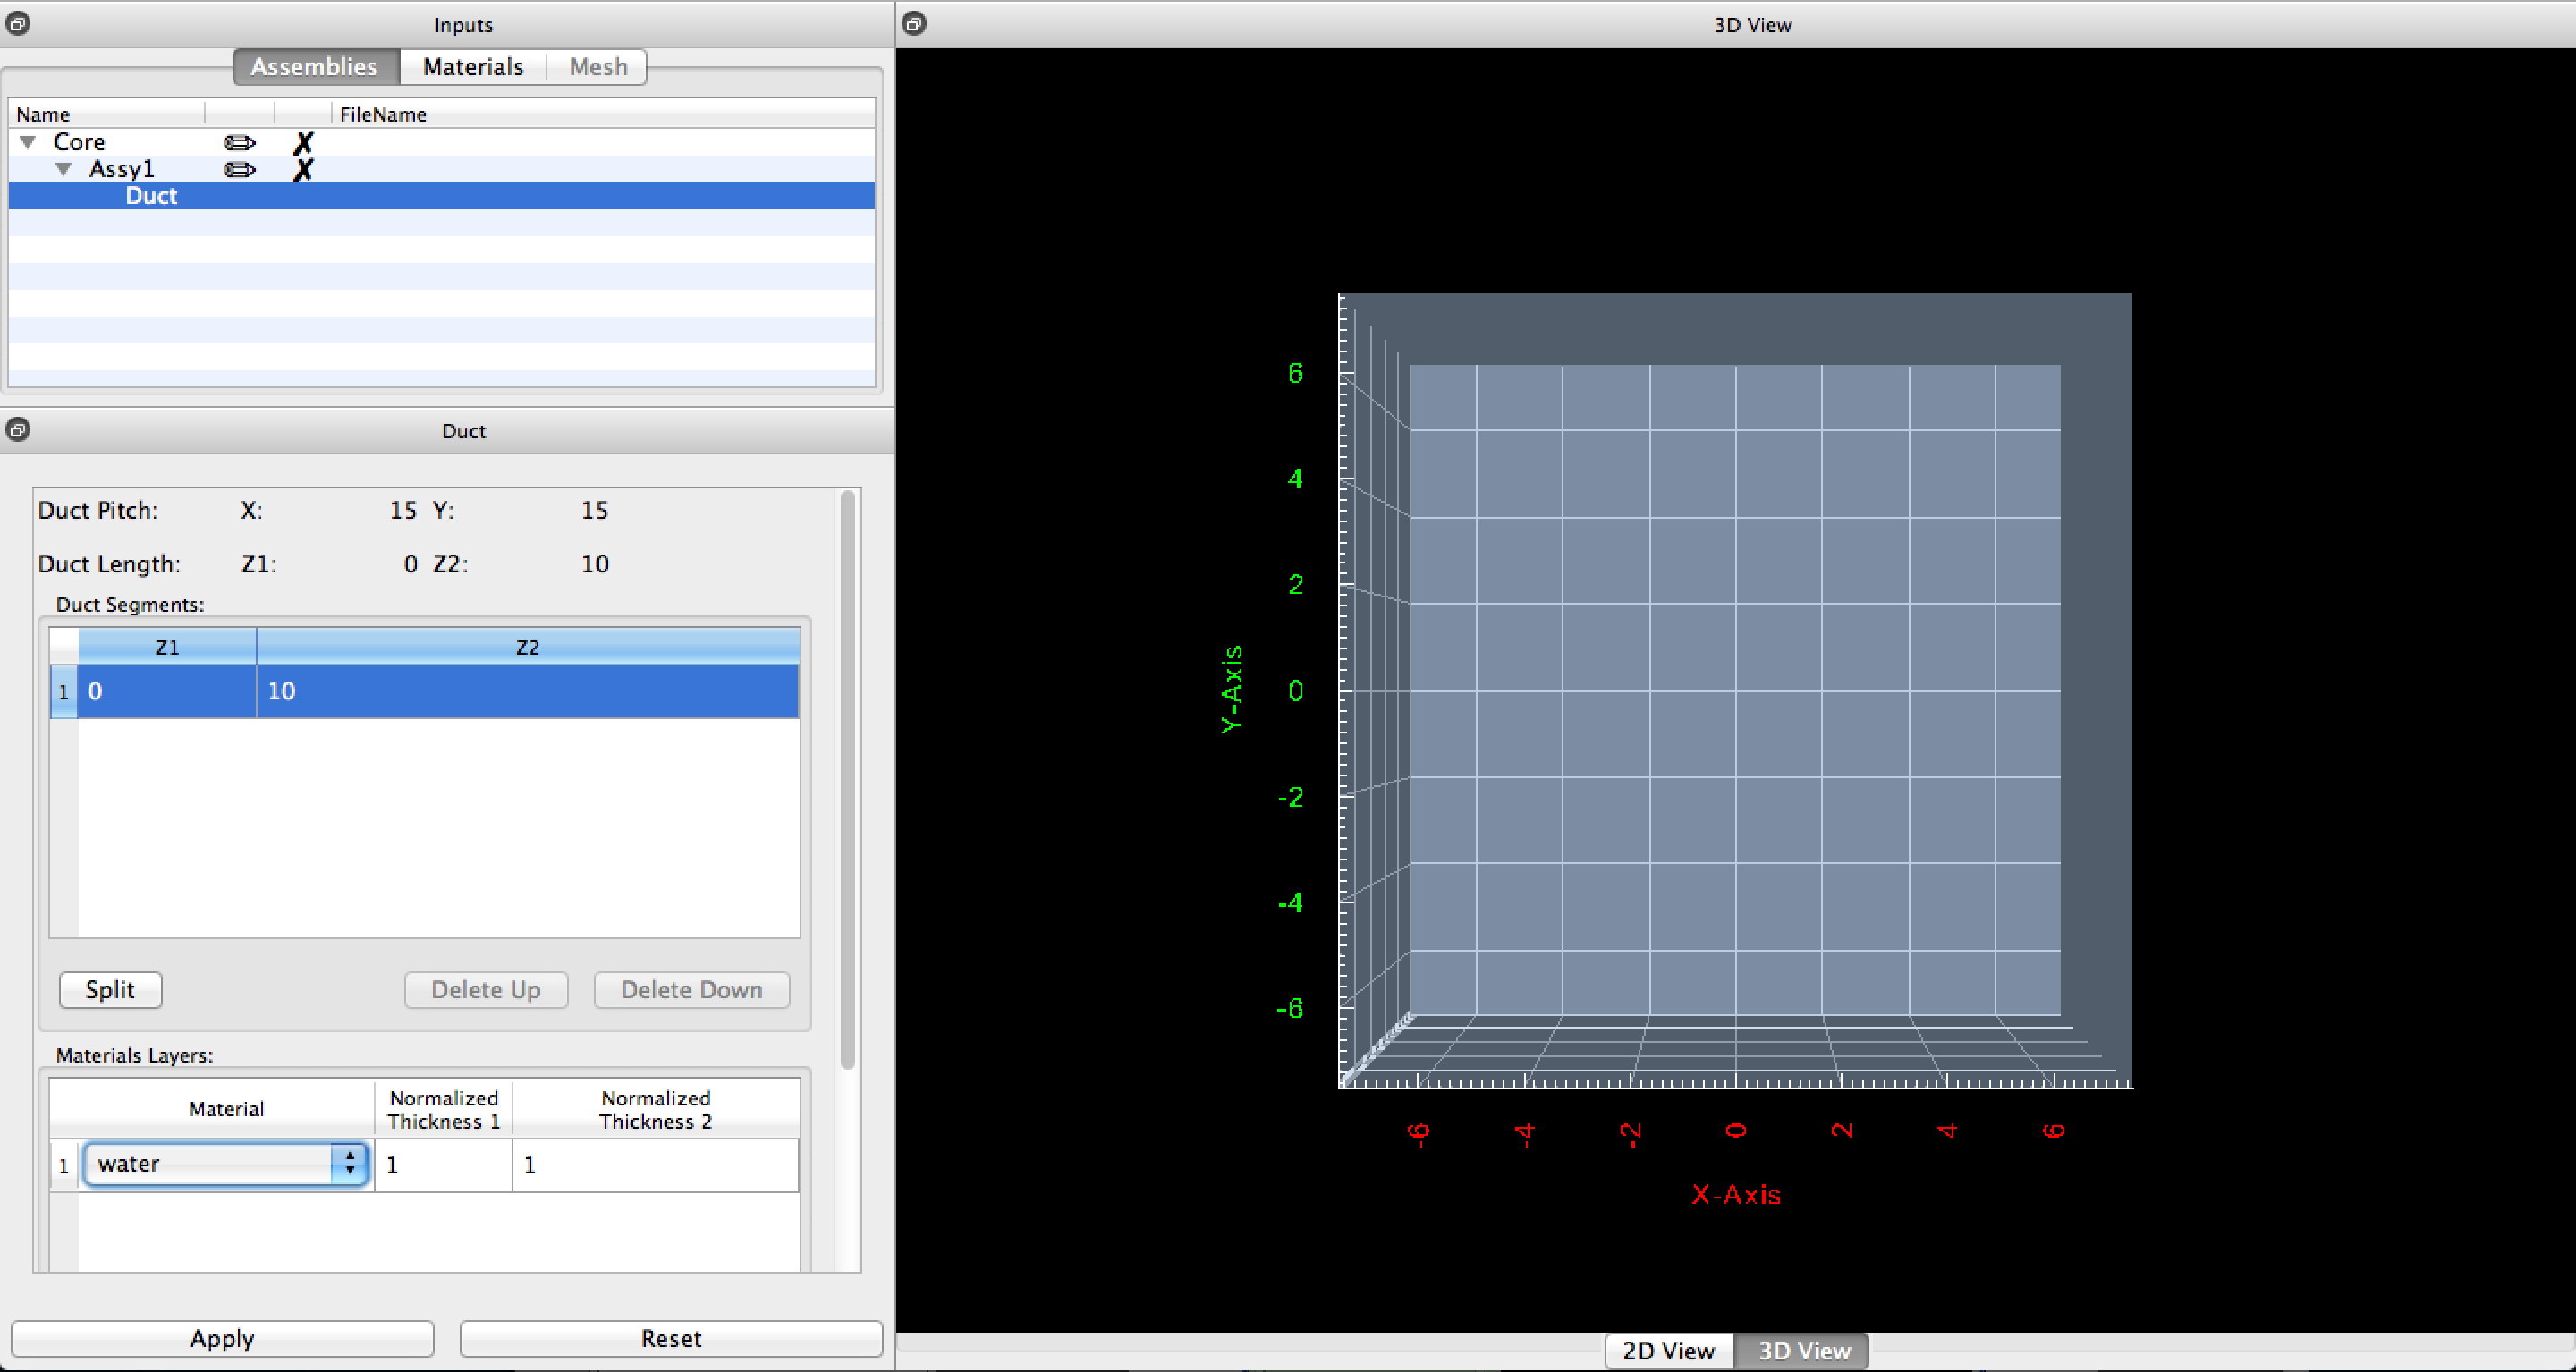
\includegraphics[width=0.9\linewidth]{Images/rect-duct-result.png}
  \caption{The final product.}
  \label{fig:rectDuctResult}
\end{subfigure}
\caption{Finished water duct.}
\label{fig:test}
\end{figure}

\clearpage

\subsection{Creating a Fuel Pin}

Right-click on the assembly and this time choose ``Create Pin''.

\subsubsection{Changing the Parameters}

Choose the dimensions of the pin to correspond to the dimensions of your duct.  In our case we have used a length of 4, corresponding to the height of the duct.

\begin{figure}[htb]
\begin{center}
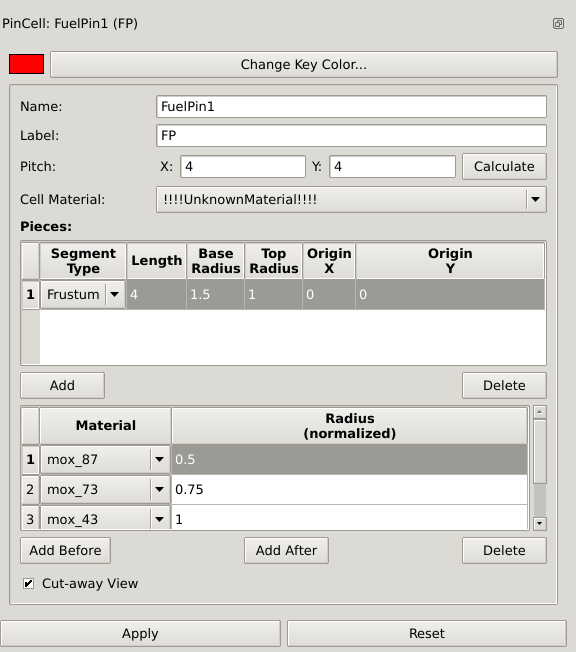
\includegraphics[width=0.4\linewidth]{Images/rect-5.png}
\caption{Fuel pin parameters.}
\label{fig:Rect5}
\end{center}
\end{figure}

Changing the key color and label is recommended, because later this will make the fuel pin more recognizeable while organizing the assembly.

\begin{wrapfigure}{r}{0.5\textwidth}
  \begin{center}
    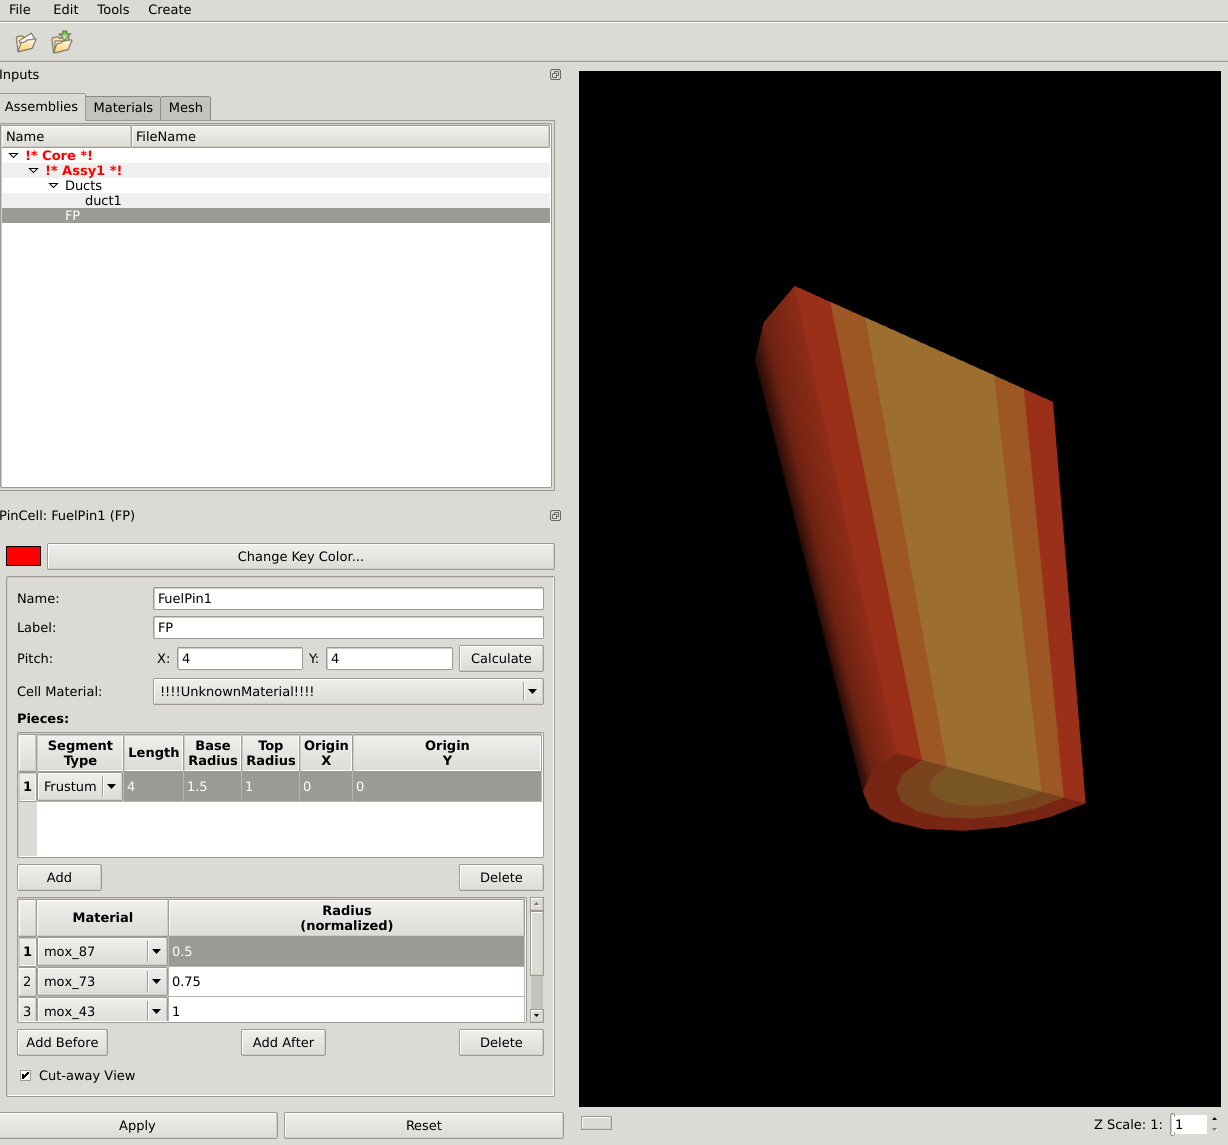
\includegraphics[width=0.48\textwidth]{Images/rect-6}
  \end{center}
  \caption{Final fuel pin product.}
  \label{fig:Rect6}
\end{wrapfigure}
Using the ``Add Before'' button, you can create a fuel pin with different layers of materials.  Refer to ~\ref{fig:Rect5} for the parameters used for our example, and ~\ref{fig:Rect6} to view the final product.

Note also the option to toggle the fuel pin's shape between a cylinder and a frustum.  The ``Cutaway view'' helps to view how the different materials are distributed within the fuel pin.

\subsection{Creating a Control Rod}
\begin{wrapfigure}{r}{0.5\textwidth}
  \begin{center}
    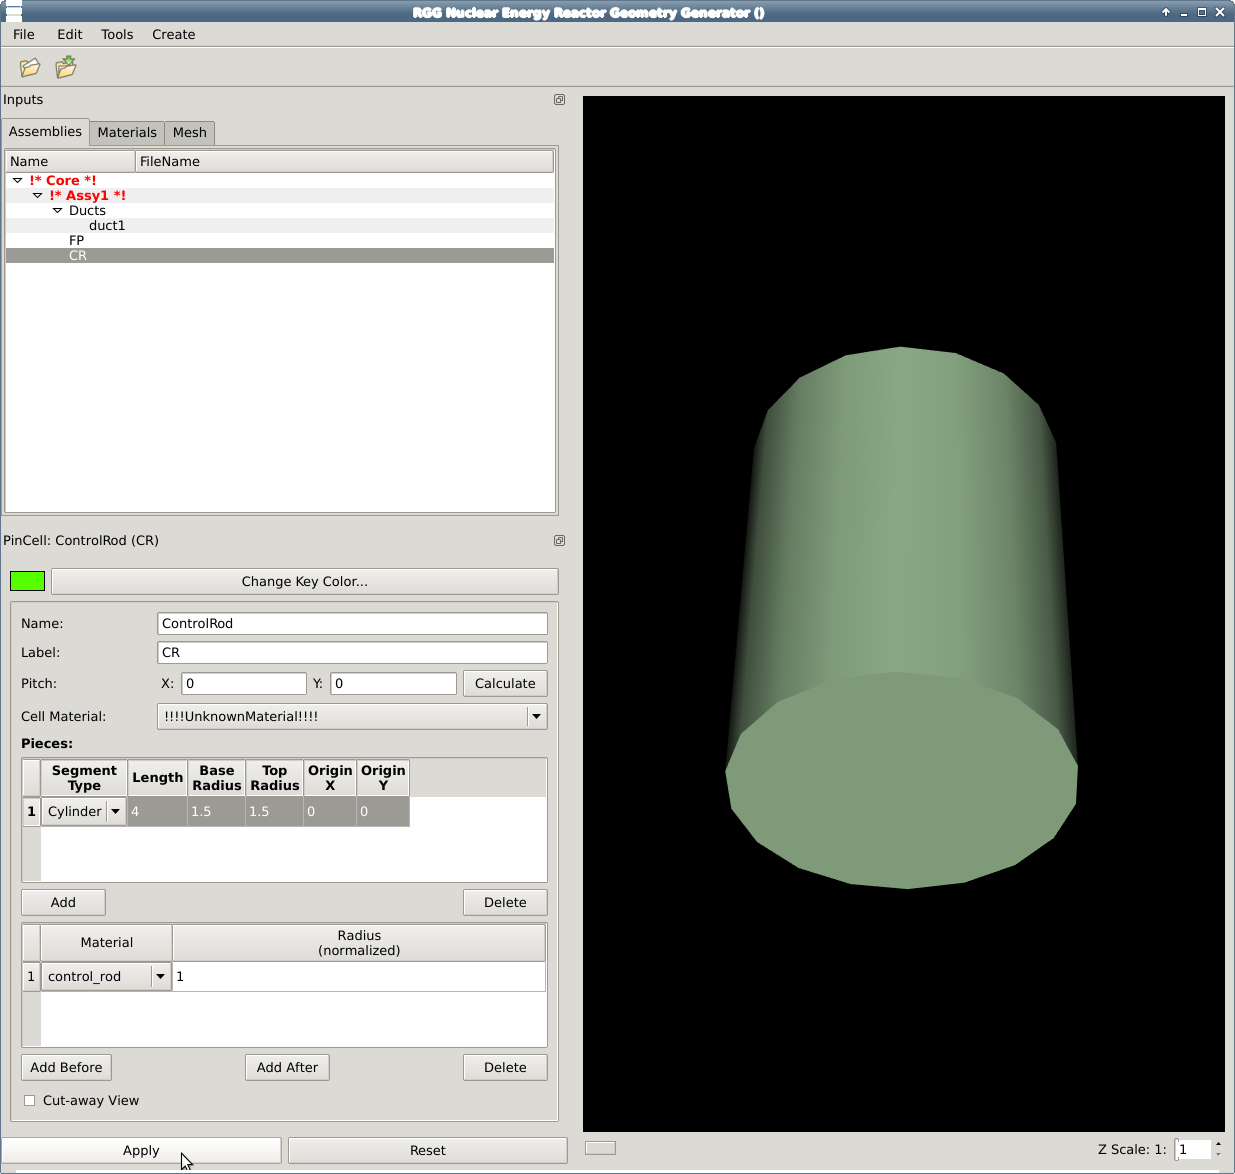
\includegraphics[width=0.48\textwidth]{Images/rect-7.png}
  \end{center}
  \caption{Final control product.}
  \label{fig:Rect7}
\end{wrapfigure}
Control rods are used to control nuclear fission. They are made out of materials which can easily absorb neutrons without undergoing fission themselves such as certain isotopes of boron, silver, or cadmium.

This is created using largely the same process as creating the fuel pin.  You can use the ``control rod'' material.  Once again, it's beneficial to change the key color to green.

Refer to ~\ref{fig:Rect7} for the final product.
\clearpage
\subsection{Adding Fuel Pins to the Assembly}

Now we want to add the pins we've created back to the assembly.  Click back on ``Assy 1'' in the assemblies view in order to see the assembly layout.  You should once again be able to see the water duct you created, and it should still be empty.  Compare your view with ~\ref{fig:Rect8}.

\begin{figure}[htb]
\begin{center}
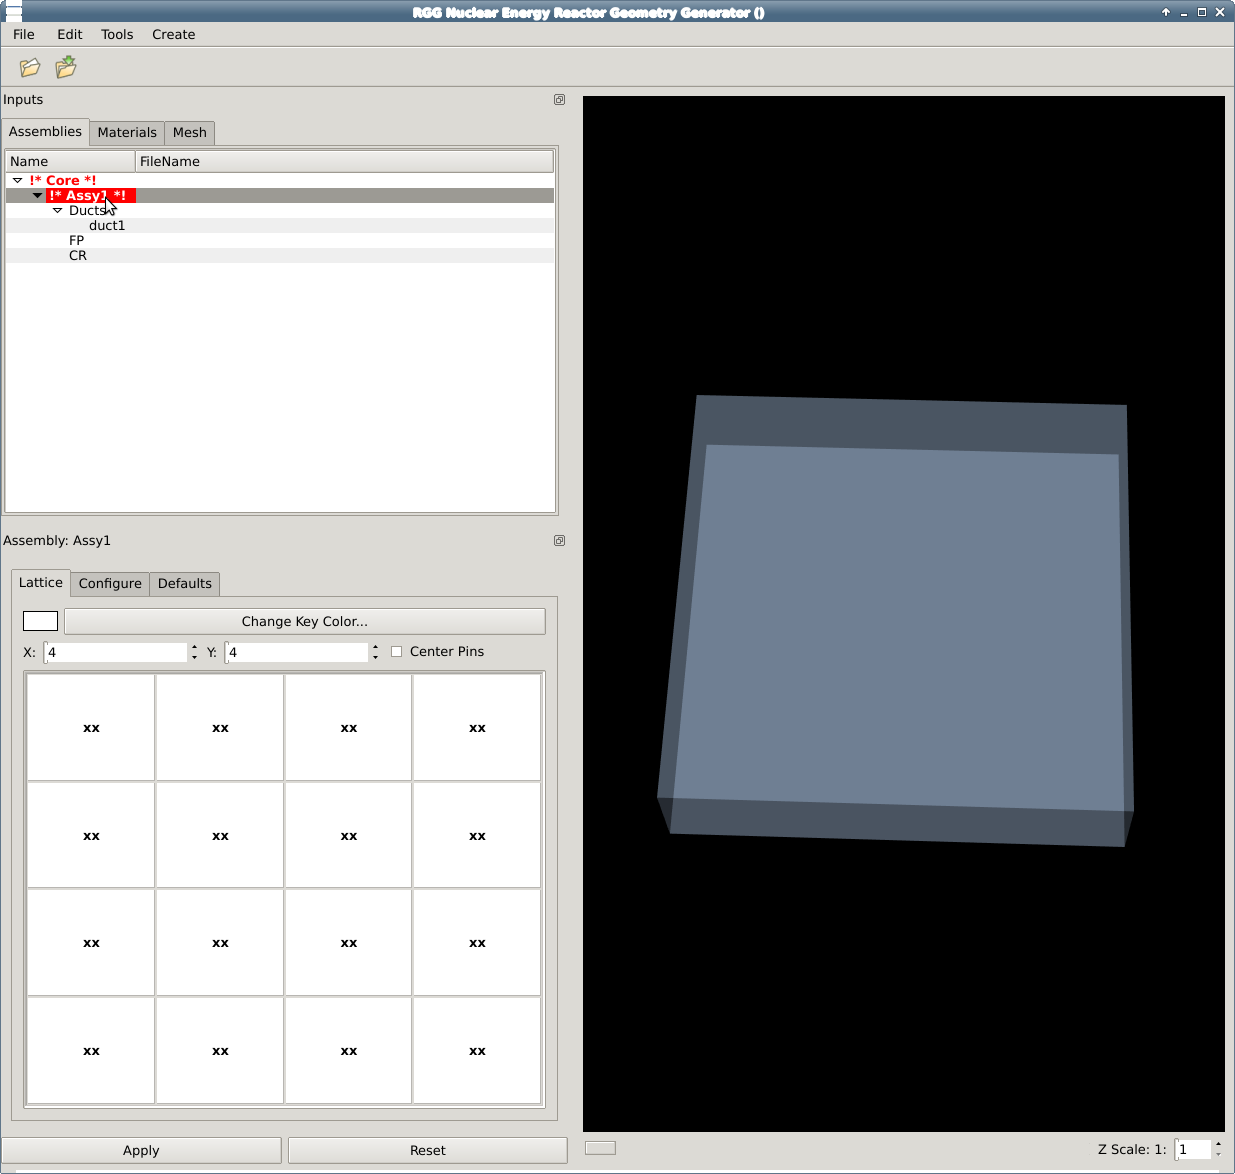
\includegraphics[width=0.4\linewidth]{Images/rect-8.png}
\caption{Empty duct in the assemblies view.}
\label{fig:Rect8}
\end{center}
\end{figure}

\begin{figure}[htb]
\begin{center}
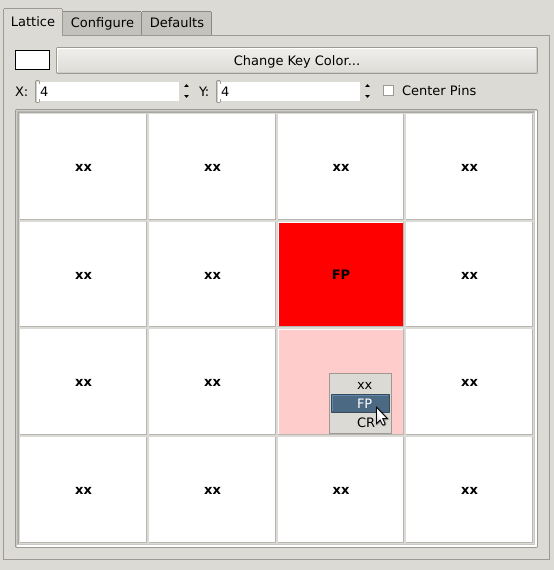
\includegraphics[width=0.4\linewidth]{Images/rect-9e1.png}
\caption{Right-click to organize the assembly.}
\label{fig:Rect9}
\end{center}
\end{figure}
Right click on each square and choose which pin to assign to it.  Alternatively, you can drag and drop pins already placed onto new squares.

In the end you should end up with something like ~\ref{fig:Rect10}.  If you find that the pins are placed in positions you didn't specify, go back to the pins and verify that the ``Pitch'' parameters are set to $X=4$ and $Y=4$ for each fuel pin and control rod.

Remember to click ``Apply'' in order to see your changes in the render window, or save them before navigating to another tab or pin.

\begin{figure}[htb]
\begin{center}
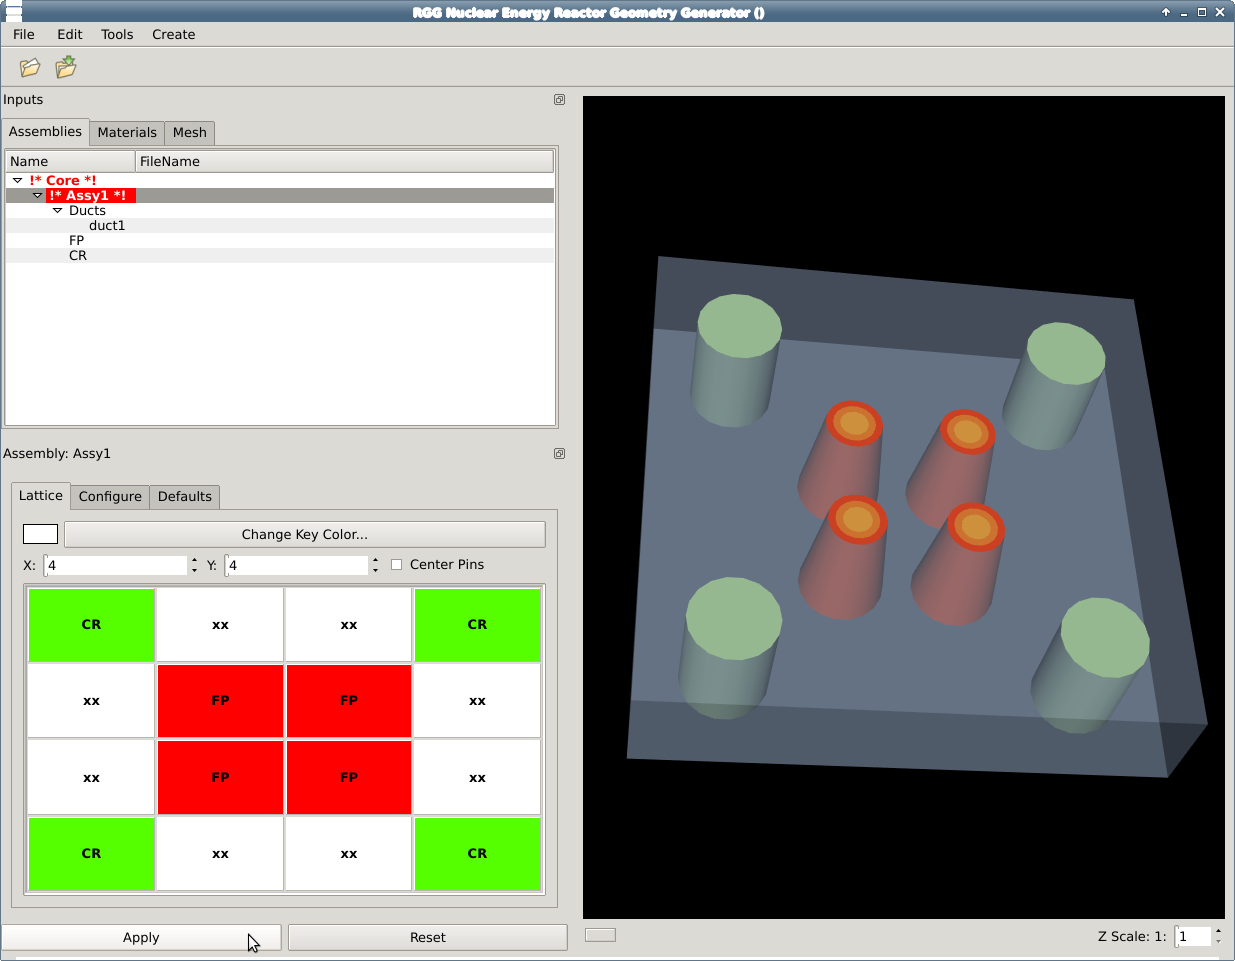
\includegraphics[width=0.7\linewidth]{Images/rect-10.png}
\caption{Final assembly.}
\label{fig:Rect10}
\end{center}
\end{figure}



\chapter{Building Hexagonal Cores}
\label{chapter:ExampleBuildingAHexagonalCore}
\section{Make a new Hexagonal Core}

First, we'll need to create a new hexagonal core.

\begin{figure}[H]
	\begin{center}
		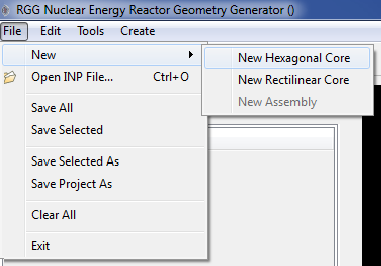
\includegraphics[width=0.5\linewidth]{Images/hex-1.png}
		\caption{Select the option to create a new hexagonal core.}
		\label{fig:Hex1}
	\end{center}
\end{figure}

The two panels on the left of the application will change.  We'll now see that the inputs panel contains an item named ``Core" with a subitem ``Assy1."  The core panel should show a hexagon labeled ``Assy1." Confirm that your application looks similar to what's shown in ~\ref{fig:Hex2}.

\begin{figure}[H]
	\begin{center}
		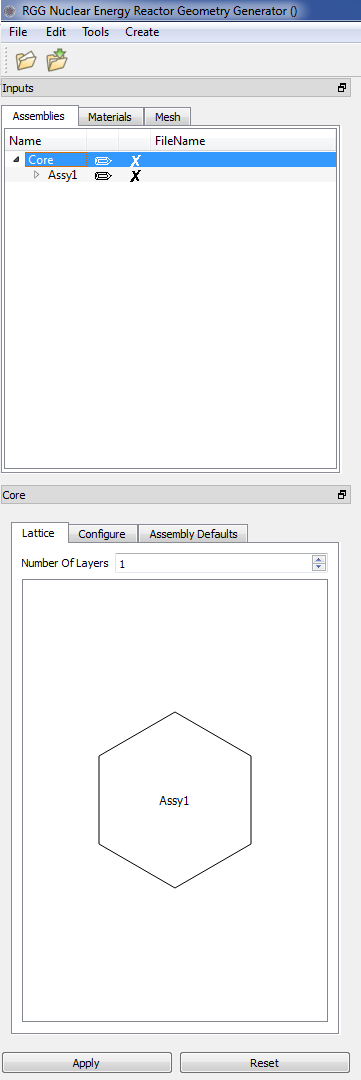
\includegraphics[width=0.2\linewidth]{Images/hex-2.png}
		\caption{The inputs and core panels after creating a new hexagonal core.}
		\label{fig:Hex2}
	\end{center}
\end{figure}

Next, we'll specify how many layers we'd like our lattice to have.  In the core panel, either type in the number of desired layers or use the buttons to the right of the field to increment and decrement the number.  The panel should look something like what's displayed in ~\ref{fig:Hex3}.

\begin{figure}[H]
	\begin{center}
		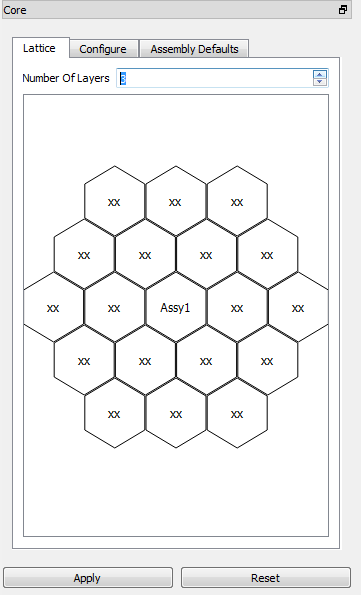
\includegraphics[width=0.5\linewidth]{Images/hex-3.png}
		\caption{Updating the number of layers of the core.}
		\label{fig:Hex3}
	\end{center}
\end{figure}

Be sure to click the apply button below to see apply changes.

\begin{figure}[H]
	\begin{center}
		
\includegraphics[width=0.5\linewidth]{Images/hex-4.png}
		\caption{The apply button.}
		\label{fig:Hex4}
	\end{center}
\end{figure}

\section{Configuring the Assembly}
\label{section:RotateAssembly30}
We need to configure the hexagonal ducts and pins we'll create to be rotated by 30 degrees to avoid interference from the different cells.  To do this, first ensure that you're clicking on the assembly we created, as shown in ~\ref{fig:Hex15}.

\begin{figure}[H]
	\begin{center}
		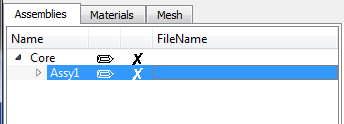
\includegraphics[width=0.5\linewidth]{Images/hex-15.png}
		\caption{Clicking on our assembly.}
		\label{fig:Hex15}
	\end{center}
\end{figure}

Then, we need to click on the configure tab in the lower panel, and scroll down to the section labeled transform.  Click the Add Rotation button.

\begin{figure}[H]
	\begin{center}
		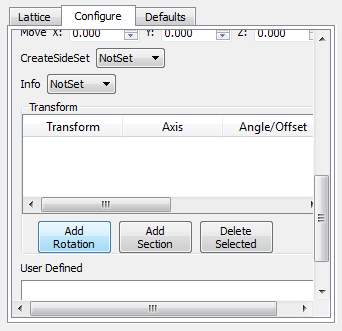
\includegraphics[width=0.5\linewidth]{Images/hex-16.png}
		\caption{Assembly transformations.}
		\label{fig:Hex16}
	\end{center}
\end{figure}

We need to change this rotation to be 30 degrees.  Enter 30 as shown in ~\ref{fig:Hex17}.

\begin{figure}[H]
	\begin{center}
		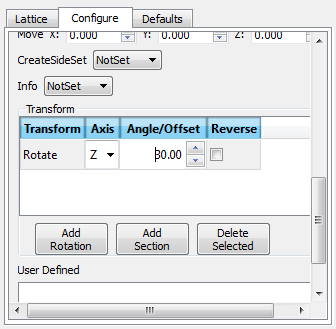
\includegraphics[width=0.5\linewidth]{Images/hex-17.png}
		\caption{Adding the 30 degree transformation.}
		\label{fig:Hex17}
	\end{center}
\end{figure}

As always, please click Apply to make sure that your changes are saved.

\section{Adding a duct to the Assembly}

\subsection{Creating the Duct}

Now that we have set up our core and configured the assembly, we need to create a duct.  To do this, follow ~\ref{fig:Hex5}.

\begin{figure}[H]
	\begin{center}
		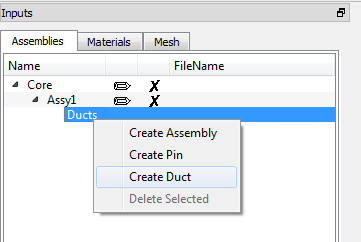
\includegraphics[width=0.5\linewidth]{Images/hex-5.png}
		\caption{Creating a duct.}
		\label{fig:Hex5}
	\end{center}
\end{figure}

Your screen should now look like this:

\begin{figure}[H]
	\begin{center}
		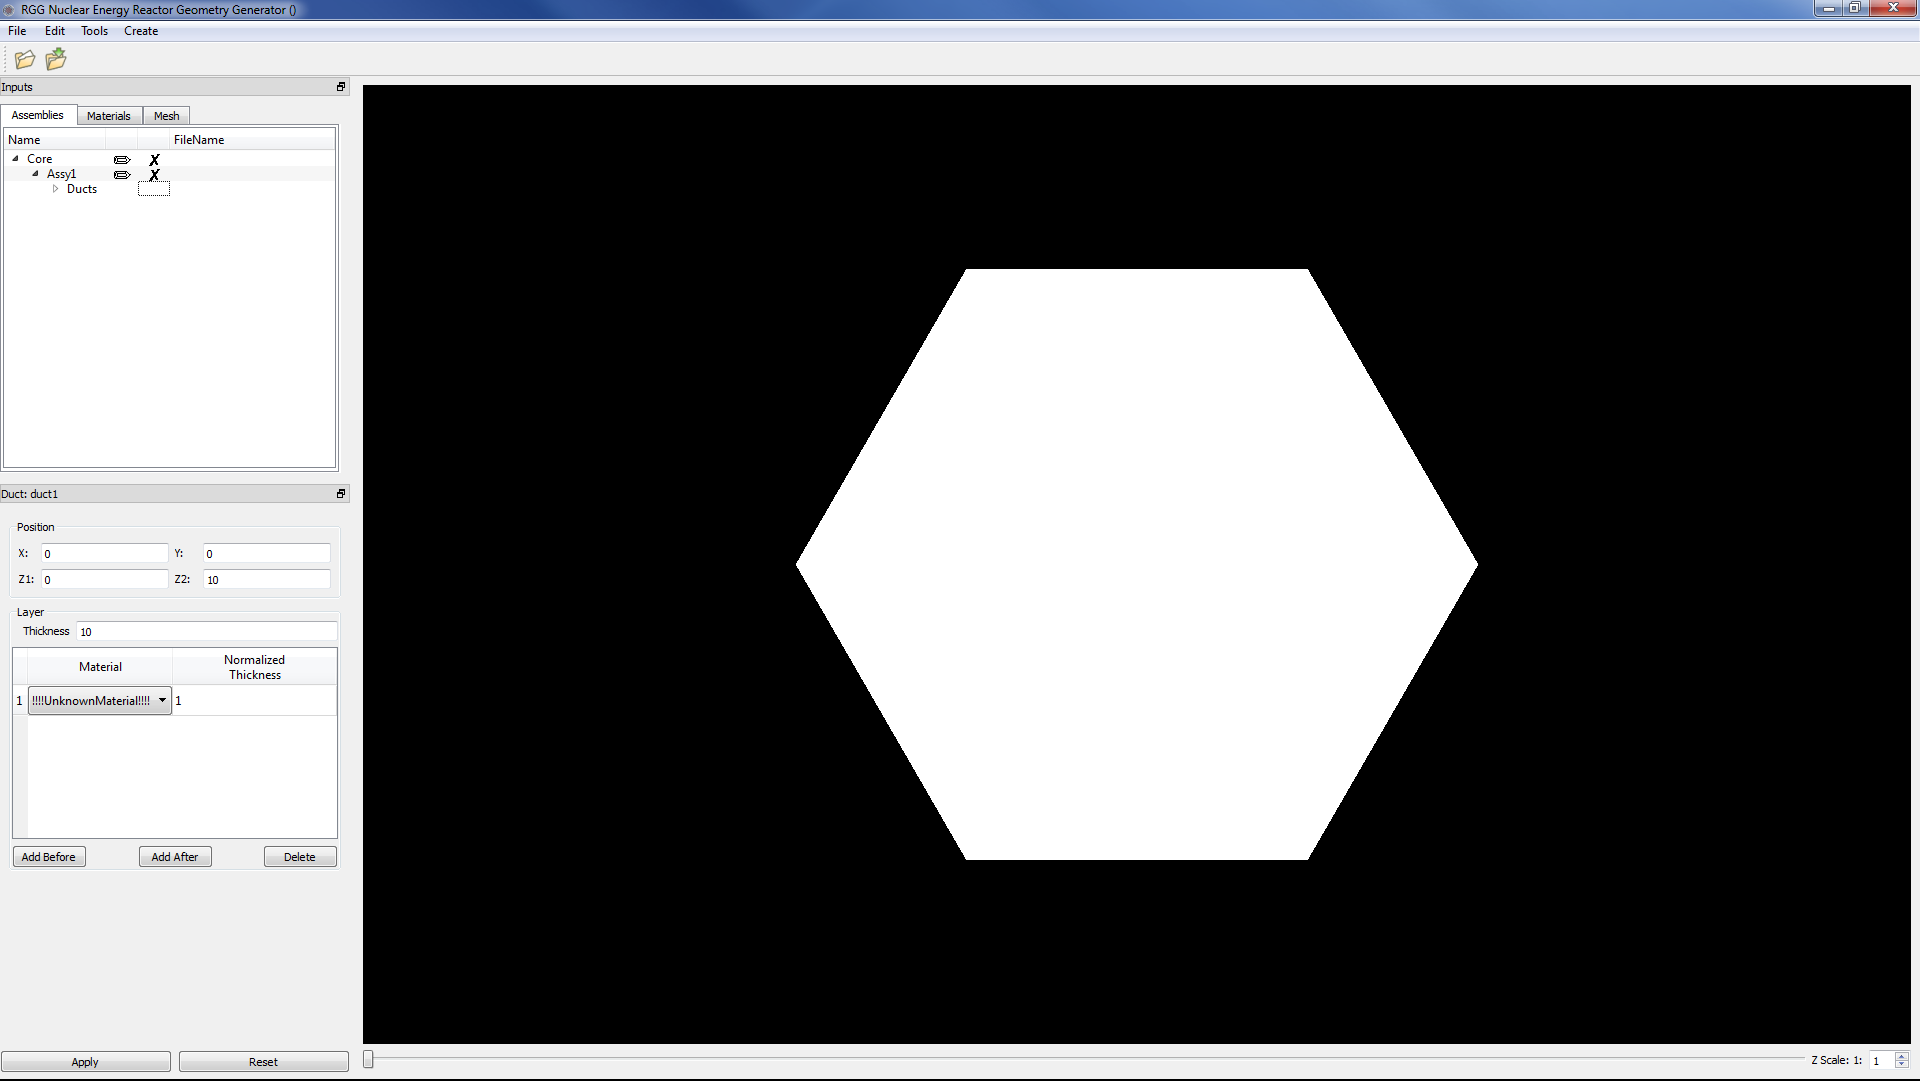
\includegraphics[width=0.85\linewidth]{Images/hex-6.png}
		\caption{Your screen after adding duct.}
		\label{fig:Hex6}
	\end{center}
\end{figure}

\subsection{Configuring Duct}

We now need to configure the duct we created.  In the inputs panel, select the duct.  This will change the lower panel to show the materials of the duct and the normalized radii of those materials.  For this duct, we'll stay simple and make the material water.  Change the material type to water by clicking the drop-down and selecting ``water."

\begin{figure}[H]
	\begin{center}
		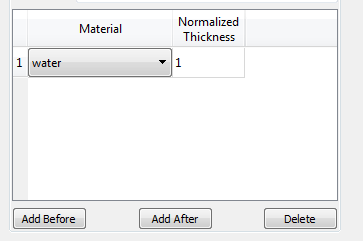
\includegraphics[width=0.5\linewidth]{Images/hex-7.png}
		\caption{Selecting water as our material.}
		\label{fig:Hex7}
	\end{center}
\end{figure}

Your screen should now look like ~\ref{fig:Hex8}.

\begin{figure}[H]
	\begin{center}
		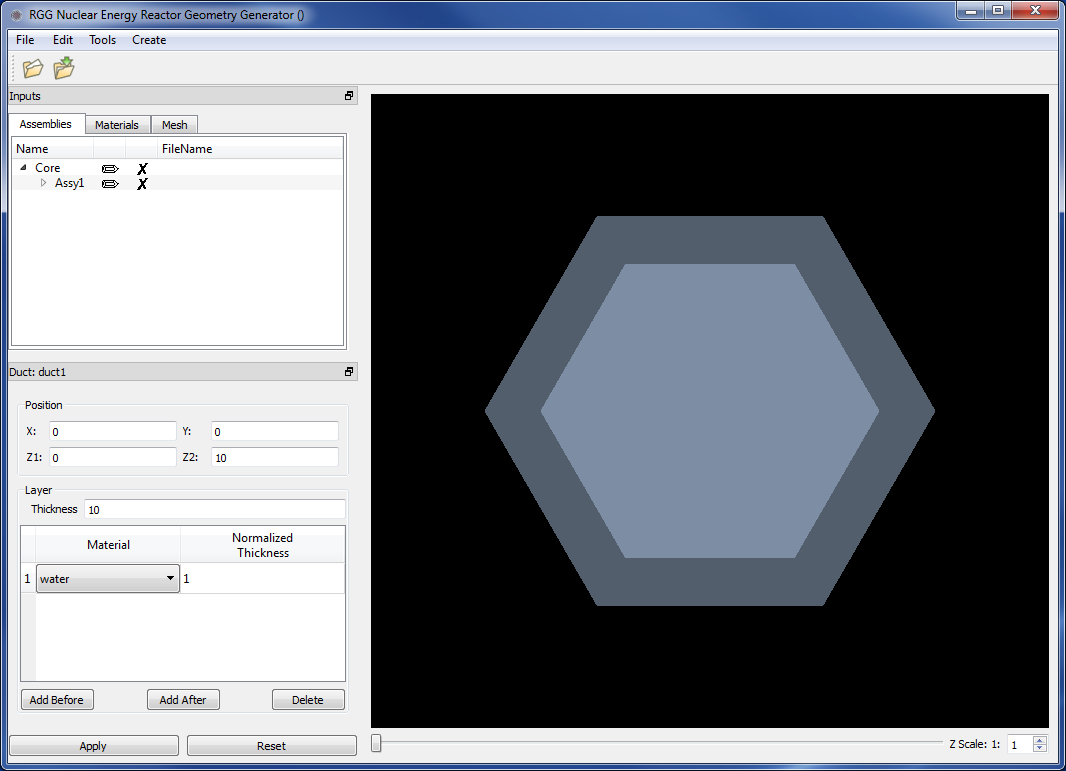
\includegraphics[width=0.5\linewidth]{Images/hex-8.png}
		\caption{Creating a duct.}
		\label{fig:Hex8}
	\end{center}
\end{figure}

\section{Adding a Pin}
\subsection{Creating a Pin}

To create a pin in the assembly, right click on the name of the assembly and select ``Create Pin."

\begin{figure}[H]
	\begin{center}
		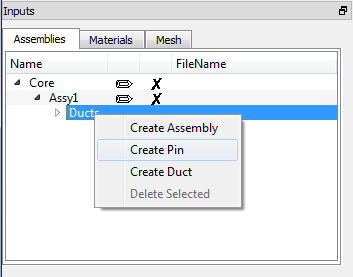
\includegraphics[width=0.5\linewidth]{Images/hex-9.png}
		\caption{Creating a pin.}
		\label{fig:Hex9}
	\end{center}
\end{figure}

\subsection{Configuring the Pin}

You can edit the name, label, pitch, and cell material of the pin.  Refer to ~\ref{fig:Hex10} to see how to change them.  We will leave them to the defaults.

\begin{figure}[H]
	\begin{center}
		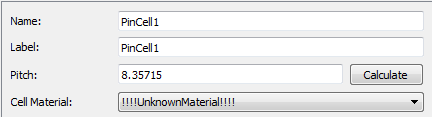
\includegraphics[width=0.5\linewidth]{Images/hex-10.png}
		\caption{Name, label, pitch, and cell material for a pin.}
		\label{fig:Hex10}
	\end{center}
\end{figure}

We now need to add pieces of the pin.  There are two kinds of pin pieces: frustrums and cylinders.  We'll add a cylinder by clicking the add button.

\begin{figure}[H]
	\begin{center}
		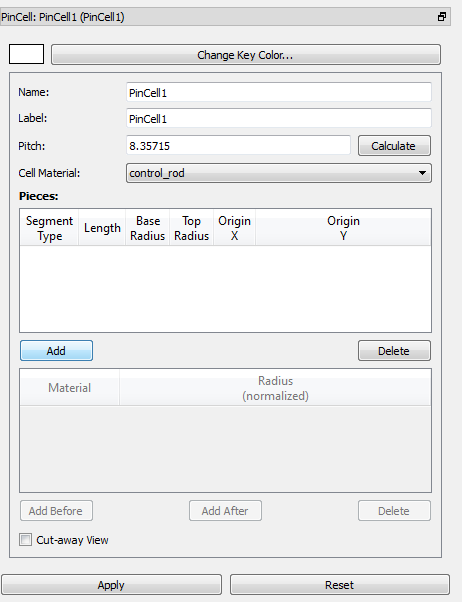
\includegraphics[width=0.5\linewidth]{Images/hex-11.png}
		\caption{Adding a pin piece.}
		\label{fig:Hex11}
	\end{center}
\end{figure}

Then, confirm that our segment type is a cylinder, and that the sum of the length of the segments is equal to the length of the duct (10).

\begin{figure}[H]
	\begin{center}
		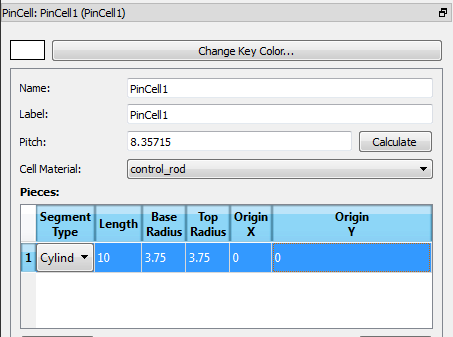
\includegraphics[width=0.5\linewidth]{Images/hex-12.png}
		\caption{Confirming our cylinder's configuration.}
		\label{fig:Hex12}
	\end{center}
\end{figure}

Now, we're going to modify the material of this cylinder.  We'll make this a control rod, so we'll change the material to match.

\begin{figure}[H]
	\begin{center}
		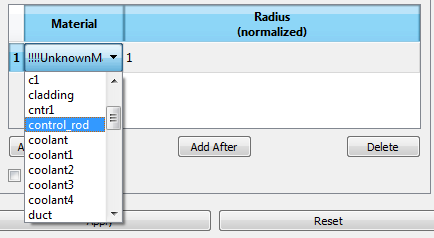
\includegraphics[width=0.5\linewidth]{Images/hex-13.png}
		\caption{Changing the material to be a control rod.}
		\label{fig:Hex13}
	\end{center}
\end{figure}

Be sure to press apply to ensure your changes go into effect.

We should see a screen like the after we're done:

\begin{figure}[H]
	\begin{center}
		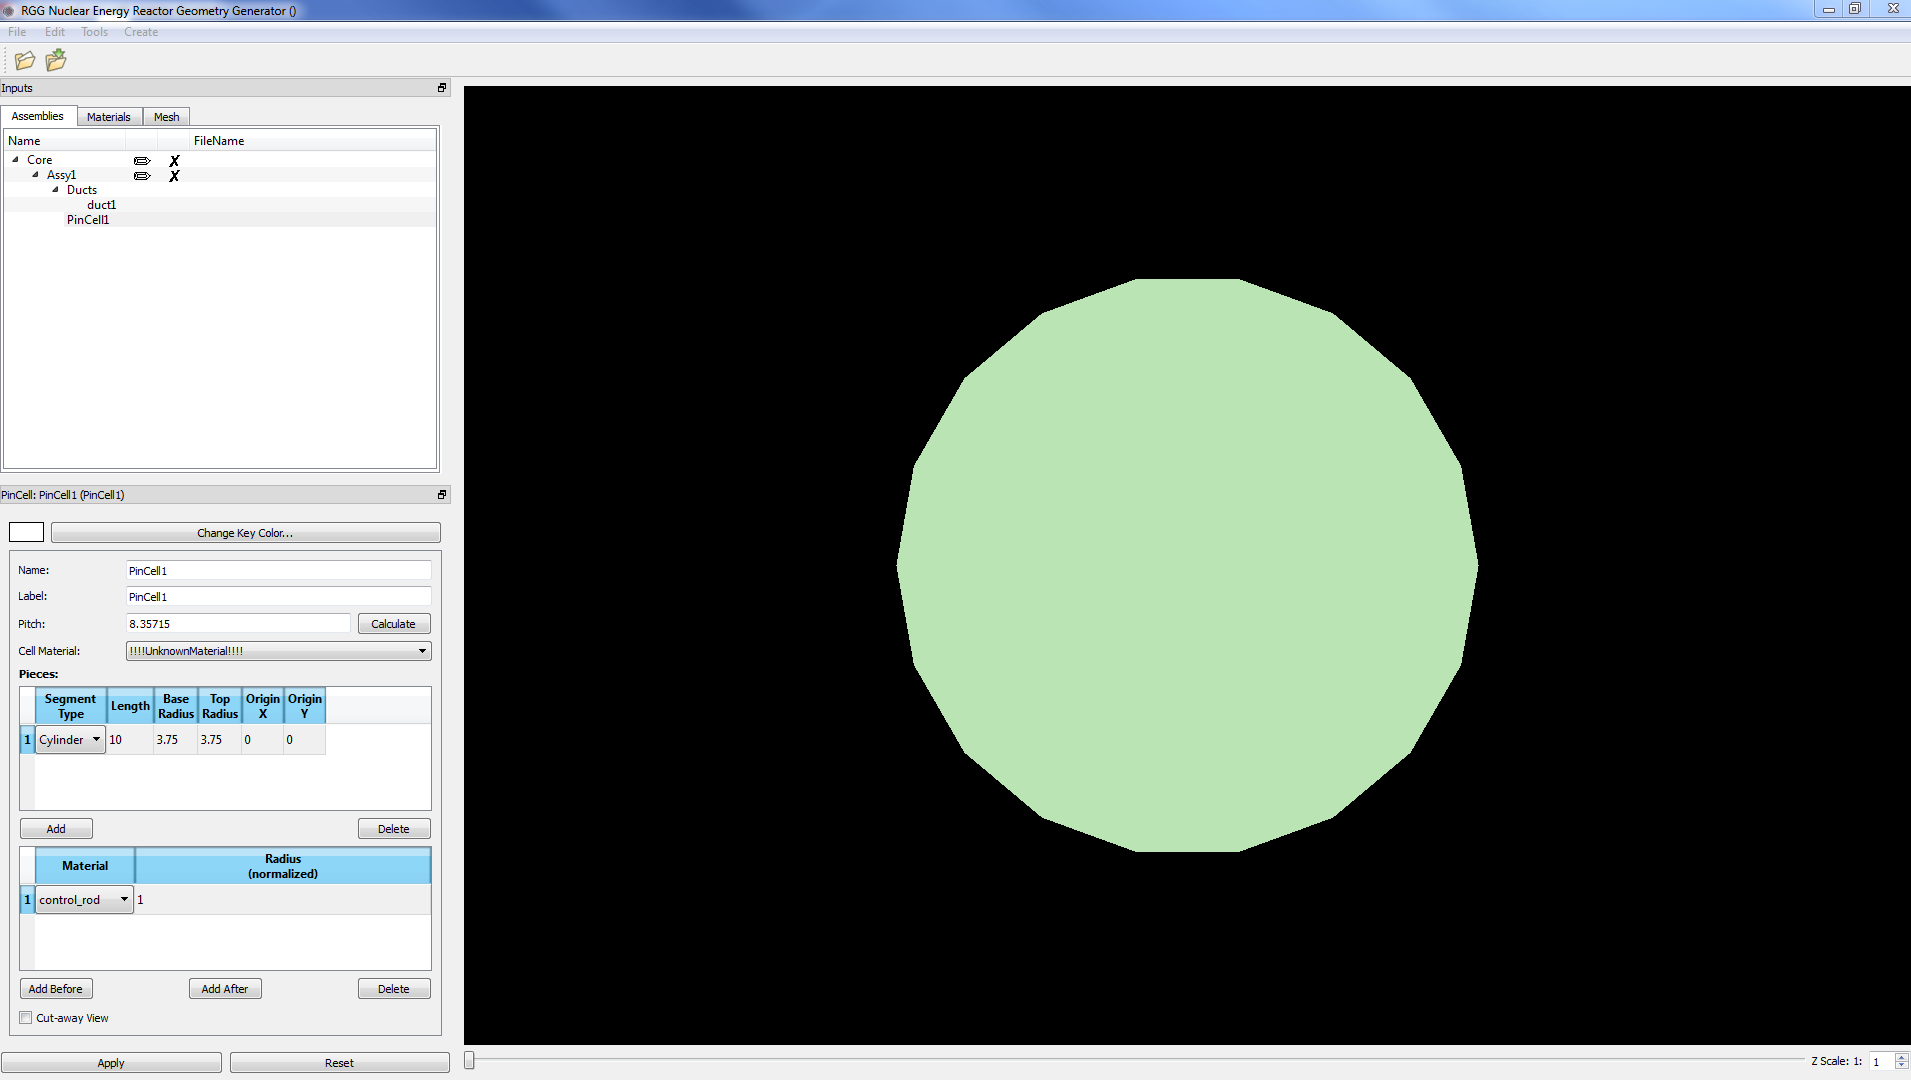
\includegraphics[width=0.85\linewidth]{Images/hex-14.png}
		\caption{After adding the cylinder.}
		\label{fig:Hex14}
	\end{center}
\end{figure}

Next, we need to add this pin to our assembly lattice.  Make sure you select ``Assy1" in the inputs menu.  Click the lattice tab in the lower panel, and right click on the hexagon to bring up a list of available pins.  Select our pin.

\begin{figure}[H]
	\begin{center}
		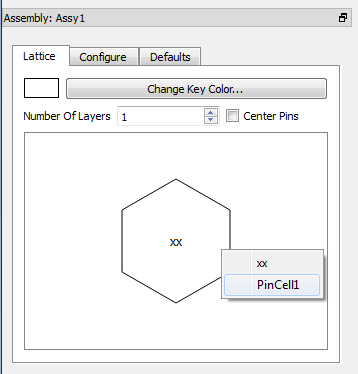
\includegraphics[width=0.5\linewidth]{Images/hex-18.png}
		\caption{Selecting our pin for the assembly.}
		\label{fig:Hex18}
	\end{center}
\end{figure}

Click the apply button to save your changes.

\section{Populating core with our assembly}

Click on our assembly (``Assy1") in the inputs pane.  In the lower pane, click on the lattice tab.  To add the assembly to any of the cells, right click to bring up a list of available assemblies, and then click on the assembly you'd like.

\begin{figure}[H]
	\begin{center}
		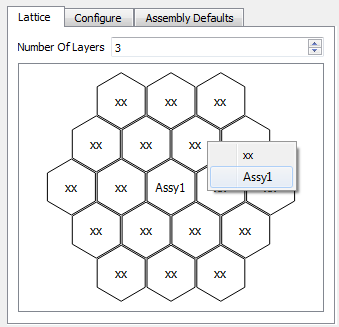
\includegraphics[width=0.5\linewidth]{Images/hex-19.png}
		\caption{Selecting assembly for a cell.}
		\label{fig:Hex19}
	\end{center}
\end{figure}

We'll select Assy1 because that's the name of the assembly we'd like.  Make sure to click the apply button to make sure that the changes we've made are applied.  Your screen should look like the following when you're done.

\begin{figure}[H]
	\begin{center}
		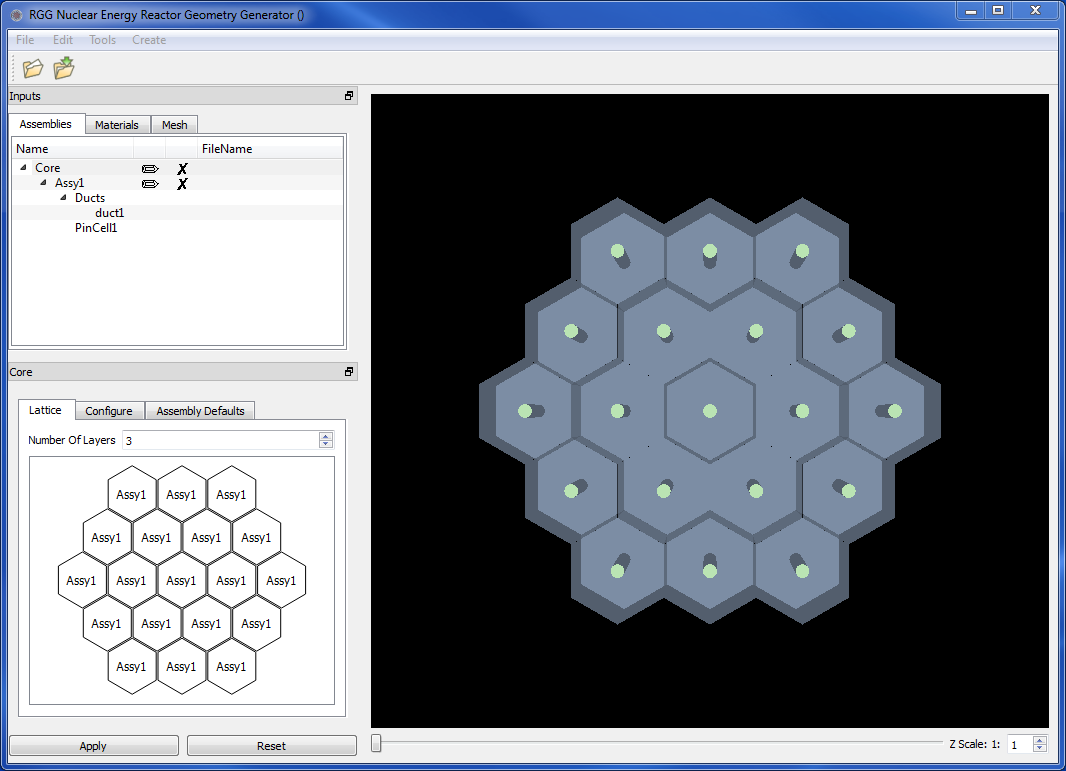
\includegraphics[width=0.85\linewidth]{Images/hex-20.png}
		\caption{Final view.}
		\label{fig:Hex20}
	\end{center}
\end{figure}

Congratulations!  You've made a hexagonal core!

\part{Reference}
\chapter{Interface Reference}
\chapter{Action Reference}

\end{document}
